\documentclass{cmspaper}
\usepackage{graphicx}
\usepackage{amsmath}
\usepackage{amssymb}
\usepackage[pdfborder=0 0 0,
            colorlinks,
            urlcolor = blue,
            linkcolor = black,
            citecolor = black,
            menucolor = black,]
           {hyperref}
%% \usepackage[colorlinks]{hyperref}
%% \usepackage{url}
\usepackage[toc,page]{appendix}
\renewcommand{\appendixname}{Appendix}
%% \renewcommand{\appendixtocname}{List of appendices}

% useful definitions

% processes
\def\dyee {\ensuremath{Z/\gamma^*\to ee}}
\def\dymm {\ensuremath{Z/\gamma^*\to\mu\mu}}
\def\dytt {\ensuremath{Z/\gamma^*\to\tau\tau}}
\def\zee {\ensuremath{Z\to ee}}
\def\zmm {\ensuremath{Z\to\mu\mu}}
\def\ztt {\ensuremath{Z\to\tau\tau}}
\def\ttbar {\ensuremath{t\bar{t}}}
\def\wwll {\ensuremath{WW\to l^+l^-}}
\def\wwlulu{\ensuremath{WW\to l^+\nu l^-\bar{\nu}}}
\def\ww {\ensuremath{WW}}
\def\wz{\ensuremath{WZ}}
\def\zz{\ensuremath{ZZ}}
\def\wgamma{\ensuremath{W\gamma}}
\def\wjets{\ensuremath{W+}jets} 
\def\tw{\ensuremath{tW}} 
\def\singletopt{\ensuremath{t} ($t$-chan)} 
\def\singletops{\ensuremath{t} ($s$-chan)} 
\def\all{all}
\def\ee{\ensuremath{ee}}
\def\emu{\ensuremath{e\mu}}
\def\mm{\ensuremath{\mu\mu}}

%units

%others
\def\pt{\ensuremath{p_T}}
\def\ipb{pb\ensuremath{^{-1}}}
\def\ifb{fb\ensuremath{^{-1}}}
\def\et{\ensuremath{E_T}}
\def\met{\ensuremath{E\!\!\!\!/_T}}
\def\fBrem{\ensuremath{f_{\rm brem}}}
\def\pin{\ensuremath{p_{\rm in}}}
\def\pout{\ensuremath{p_{\rm out}}}


\setcounter{topnumber}{1}
\setcounter{bottomnumber}{1}

\begin{document}
\begin{titlepage}

  \analysisnote{2011/XXX}

  \date{\today}

  \title{Search for Higgs boson in WW to di-lepton final state}

  \begin{Authlist}
  \end{Authlist}

  % if needed, use the following:
  \collaboration{CMS collaboration}

  % \Anotfoot{a}{On leave from prison}
  %\Anotfoot{b}{Now at the Moon}
  \begin{abstract}
    This note describes a search for the Higgs boson in WW$\to$ll
    final state with xx~fb$^{-1}$ of $pp$ collision data at $\sqrt s =
    $ 10~TeV. We look for Higgs events in $ee$, $\mu\mu$ and $e\mu$
    channels with 0, 1 and 2 jets in the final state.
  \end{abstract} 

\end{titlepage}
\tableofcontents
%\listoftables
%\listoffigures
\newpage 

\section{Introduction}
  \label{sec:overview}
%  \input{overview}
\section{Data samples}
  \label{sec:dataset}
%  \input{dataset}
\section{Event selection}
  \label{sec:selection} 
%  In this section we define the common objects and preselection requirements 
used by all of the approaches considered in this analysis.

The fully leptonic final state consistens of two isolated leptons
and large missing energy from the two undetectable neutrinos.
This is the same final state as the non-resonant $\WW$ background.
The Higgs cross-section is several orders of magnitude lower than
the major reducible background processes: \ttbar{}, \wjets{} and Drell-Yan. 
We thus perform several steps to select and extract the Higgs boson signal from data:

\begin{enumerate}
    \item We select events that pass pre-defined lepton triggers
    \item We then select those with the final state described above:
        \begin{itemize}
            \item Two opposite charge leptons ($ee$, $\mu\mu$, $e\mu$)
            \item $\pt>20~\GeVc$ for the leading lepton and $\pt>10~\GeVc$ for the trailing lepton.
            \item Standard identification and isolation requirements
        \end{itemize}    
    \item We apply a common $\WW$ preselection with no restriction on the number of reconstructed jets
    \item Finally, we perform two \emph{Higgs mass dependent} event selections; one cut-based and one using a multivariate technique. 
\end{enumerate}

These steps are now described in detail.


  \subsection{Trigger}
    \label{sec:sel_trigger}
%    Triggering on Higgs boson decays in the dilepton final state increases 
in difficulty with increasing instantaenous luminosity.
Single lepton triggers can only be sustained with very tight identification and
isolation requirements and large transverse momentum thresholds.
This means that double lepton triggers are the only viable option to maintain
sensitivity to a low mass Higgs boson, where the leptons transverse momentum
can be small.

We designed a suite of signal and control triggers appropriate for this analysis.
These dilepton triggers have a high efficiency to collect Higgs boson events
and are sufficiently loose to collect control events to estimate
fake lepton backgrounds and selection efficiencies with adequate precision. The detailed 
trigger paths were described in~\cite{HWW2011}.

  \subsection{Muon selection} 
    \label{sec:sel_muons}
%    Muons in CMS are reconstructed as either $StandAloneMuons$ (track
in the muon detector with low momentum resolution), $GlobalMuons$
(outside-in approach seeded by a $StandAloneMuon$ with a global fit
using hits in the muon, silicon strip and pixel 
detectors) and $TrackerMuons$ (inside-out approach seeded by an offline 
silicon strip track, using the muon detector only for muon identification 
without refitting the track). Most good quality muons are reconstructed as 
all three types at the same time and the momentum resolution is dominated by the inner
tracker system up to about 200~$\GeVc$ in transverse momentum. Details about the
optimization at low $\pt$ are given in Appendix~\ref{app:mus}. The specific
requirements to select good prompt isolated muons are the following:
\begin{itemize}
\item the muon must be found by both the global and tracker muon algorithms;
\item the global muon must have at least one good muon hit;
\item the tracker muon must have at least two matches to muon segments in 
      different muon stations;
\item more than 10 hits in the inner tracker;
\item at least one pixel hit;
\item $\chi^2/{\mathrm{ndof}} < 10$ on a global fit;
\item impact parameter in the transverse plane $|d_{0}| < 0.02~(0.01)$~cm for
      muons with $\pt$ greater (smaller) than 20 $\GeVc$,
      calculated with respect to the primary vertex;
\item longitudinal impact parameter $|d_{z}| <0.2$~cm,
      calculated with respect to the primary vertex;
\item pseudorapidity $|\eta|$ must be smaller than 2.4;
\item relative \pt\ resolution is better than 10\%.
\end{itemize}

Furthermore, the particle flow candidate-based isolation variable is 
used to reduce the contamination from the non-isolated muons originating from
jets. 

\begin{itemize}
\item $\rm{Iso}_{PF}$: defined as the scalar sum of the \pt\ of the 
    particle flow candidates satisfying the following requirements:
    \begin{itemize}
    \item $\Delta R~<~0.3$ to the muon in the $\eta \times \phi$ plane,
    \item $|d_{z}(\mathrm{PF Candidate}) - d_{z}(\mathrm{muon})| < 0.1$~cm, if the PF candidate is charged,
    \item \pt $>1.0$ GeV, if the PF candidate is classified as a neutral hadron or a photon.
    \end{itemize}
\end{itemize}

We require $\frac{\rm{Iso}_{PF}}{\pt}~<~0.13~(0.06)$ for muons in the barrel 
with $\pt$ greater (smaller) than 20 $\GeVc$. For muons in the endcap, we
require $\frac{\rm{Iso}_{PF}}{\pt}~<~0.09~(0.05)$ for muons with $\pt$ 
greater (smaller) than 20 $\GeVc$. Further details of the choice of
the isolation requirement is documented in Appendix \ref{app:pfIsoStudy}.


  \subsection{Electron selection} 
    \label{sec:sel_electrons}
%    We select electrons using a cut-based approach consistent with the electron 
selection criteria used for the measurement of the inclusive W and Z 
cross-section~\cite{VBTFCrossSectionNote}. In order to deal with large 
background rates at low electron momentum, we developed a few additional 
requirements. The choice of the electron selector type and the optimization procedure
are described in Appendix~\ref{app:els}.

Electrons are required to have transverse momentum larger than $15$ GeV and $|\eta| < 2.5$. 
Electron identification is based on selection cuts on shower shape ($\sigma_{i\eta i\eta}$), 
track to cluster matching ($\Delta \phi_{\mathrm{in}}$ and $\Delta \eta_{\mathrm{in}}$), and the amount 
of relative hadronic activity (H/E). 
For electrons with $p_T<$20 GeV, the selection is tightened by adding a cut on the fraction of momentum 
loss due to radiation (fbrem) and on the ratio between the SuperCluster energy and the track momentum ($E/p$).
The electron is required to be isolated by imposing a requirement on the combined relative isolation 
($\rm{Iso}_{Track}$, $\rm{Iso}_{ECAL}$, $\rm{Iso}_{HCAL}$ in a $\Delta$R $< 0.3$ cone / $p_{T}$), 
where $\rm{Iso}_{ECAL}$ is calculated using ECAL crystals and additional vetos have been 
applied to remove tracks and ECAL crystals from the isolation sums to better account for 
the electron footprint~\cite{ElIso}. In the barrel region ($|\eta| < 1.479$) we subtract 1~GeV of 
ECAL energy deposition if it is more than 1~GeV to account for the noise pedestal. 
In order to veto fake electrons from converted photons, we look for a reconstructed conversion vertex where 
one of the two track is compatible with the electron~\cite{ConversionNote}, 
and require that there are no missing expected hits forming the electron track~\cite{ConversionNote},~\cite{NExpHits}. 
Finally we impose cuts on the transverse and longitudinal impact parameters with
respect to the primary vertex to reduce fake electrons from non-prompt
sources. Cut values are summarized in Tab.~\ref{tab:electronSelection}.

\begin{table}[!ht]
\begin{center}
\begin{tabular}{|c|c|c|}
 \hline
 \multicolumn{3}{|c|}{Identification $p_T>$20 GeV} \\
\hline
 Cut Variable           &   Cut Value (Barrel)                   & Cut Value (Endcap)    \\
\hline
 $\sigma_{i\eta i\eta}$      &   $<0.01$                              & $<0.03$               \\ 
 $\Delta\phi_{\mathrm{in}}$  &   $<0.06$                              & $<0.03$               \\ 
 $\Delta\eta_{\mathrm{in}}$  &   $<0.004$                             & $<0.007$               \\ 
 H/E                         &  $<0.04$                          &   -          \\ 
 \hline
 \hline
 \multicolumn{3}{|c|}{Identification 15$<p_T<$20 GeV} \\
\hline
 Cut Variable           &   Cut Value (Barrel)                   & Cut Value (Endcap)    \\
\hline
 $\sigma_{i\eta i\eta}$      &   $<0.01$                              & $<0.03$               \\ 
 $\Delta\phi_{\mathrm{in}}$  &   $<0.03$                              & $<0.02$               \\ 
 $\Delta\eta_{\mathrm{in}}$  &   $<0.004$                             & $<0.005$               \\ 
 H/E                       &  $<0.025$                          &   -          \\ \hline
 Additional cut           &  \multicolumn{2}{|c|}{$fbrem>0.15~OR~(|\eta|<1~AND~E/p>0.95)$} \\ 
 \hline
 \hline
 \multicolumn{3}{|c|}{Isolation and Impact Parameter} \\
\hline
 Combined relative isolation &  $<0.1$                           &  $<0.1$              \\
 transverse impact parameter $|d_{0}|$  &  $<0.02$ cm   & $<0.02$ cm    \\
 longitudinal impact parameter $|d_{z}|$  &  $<0.2$ cm   & $<0.2$ cm    \\
 \hline
 \hline
 \multicolumn{3}{|c|}{Conversion Rejection} \\
 \hline
 Missing hits in inner pixel layers  &   $=0$      &  $=0$           \\ 
 $N_{hits}$ before vertex       &  $=0$    &   $=0$      \\  
 Vertex fit probability       &  $>10^{-6}$    &   $>10^{-6}$      \\  
 Transverse vertex distance from PV       &  $>2.0$ cm    &   $>2.0$ cm      \\  
 \hline

\hline
\end{tabular}
\caption{Summary of the electron selection requirements. \label{tab:electronSelection}}

\end{center}
\end{table}

  \subsection{Missing \et} 
    \label{sec:sel_met}
%    
The missing transverse energy is used to reject background events
where there is no natural source of missing energy, primarily Drell-Yan events. 

In the presence of high multiple-interactions (pile-up), the instrumental \met\ tail in 
$\dyll$ events increases significantly.  To improve the signal over background performance of \met\ selections 
in the presence of pile-up, we make use of the ``trk-MET''~\cite{trkMET}, constructed from 
charged particles consistent with originating from the primary vertex. 

The event $\met$ trk-MET is defined as 
\begin{equation}
\text{trk-MET} \equiv -\overrightarrow{p_T}(l_1) - \overrightarrow{p_T}(l_2) - \sum_i{\overrightarrow{p_T}(i)}, \\
\label{eq:trkmet}
\end{equation}

where $\overrightarrow{p_T}(l_1)$ and $\overrightarrow{p_T}(l_2)$ are the transverse momentum vectors of the two 
leptons passing the lepton selections described in Sec.~\ref{sec:sel_muons} and Sec.~\ref{sec:sel_electrons}, 
and $\overrightarrow{p_T}(i)$ represent the tranverse momentum vectors of the charged PFCandidates satisfying the following requirements:
%%%%%%%%%%%%%%%%%%%%%%%%%%
\begin{itemize}
\item the track matched to PFCandidate has $\Delta z < 0.1$~cm with respect to the signal primary vertex;
\item the track has $\Delta R > 0.1$ with respect to both leptons, to avoid double-counting of the leptons.
\end{itemize}
%%%%%%%%%%%%%%%%%%%%%%%%%%


These two variations of \met\ are weakly-correlated in $\dyll$ background, and 
strongly correlated for the signal processes with geninue $\met$, as shown in Figure~\ref{fig:met_scatter}. 
Therefore the signal over background ratio is improved if we select the events 
based on the mininum of these two projected $\met$ values, $\text{min-MET} \equiv min(\text{trk-MET}, \text{PFMET})$. 


%%%%%%%%%%%%%%%%%%%%%%%%%%%%%%%%%%%%%%%%%%%
\begin{figure}[hbt]
\begin{center}
\includegraphics[width=1\linewidth]{figures/met_scatter.pdf} 
\caption{\label{fig:met_scatter}\protect Distributions of trk-MET vs. pfmet in data (left), 
$\dyll$ MC (center) and Higgs $\rightarrow$ WW MC (right).}
\end{center}
\end{figure}
%%%%%%%%%%%%%%%%%%%%%%%%%%%%%%%%%%%%%%%%%%%


  \subsection{Jet counting} 
    \label{sec:sel_jets}
%    %To split the analysis in different jet bins, we count events 
%containing jets with $\pt > ~30~\GeV$ within $|\eta|<5.0$. 

Jets are reconstructed using calorimeter and tracker information using a particle flow 
algorithm~\cite{jetpas}. The anti-${\rm k_T}$ clustering algorithm~\cite{antikt} 
with ${\rm R=0.5}$ is used. We apply the standard jet energy 
corrections~\cite{jes} to the reconstructed jets, where the L1 Fast Jets 
corrections are included. The latter corrections are rather important since 
they help in flatening the reconstruction efficiency as a function of the 
number of overlapping events.
To exclude electrons and muons from the jet sample, these 
jets are required to be separated from the selected leptons in $\Delta R$ 
by at least $\Delta R^{\mathrm{jet-lepton}}>0.3$.

In this analysis we use high $p_T$ jets to define the analysis jet bin
and low $p_T$ jets to do the top events veto.
We define:
\begin{itemize}
\item {\it counted jet}: a reconstructed jets with $\pt > ~30~\GeV$ within $|\eta|<5.0$;
\item {\it low $p_T$ jet}: a reconstructed jets with $7~ <\pt < ~30~\GeV$ within $|\eta|<5.0$
\end{itemize}

We analyze the events separately based on the number of counted jets
in the event.

%In the 0-Jet bin, the performance of the jet veto 
%is validated on data using Drell-Yan events, 
%as will be explained in Sec.~\ref{sec:backgrounds}. 

  \subsection{$Z$ veto}
    \label{sec:sel_zveto}
%    To further reduce the Drell--Yan background in the $\Ep\Em$ and $\Mp\Mm$ final
states, we veto events with a dilepton invariant mass within $15~\GeV$ of the $\Z$.
We also reject events with a dilepton invariant mass below $12~\GeVcc$
to suppress contributions from low mass resonances.

  \subsection{Top tagging}
    \label{sec:sel_toptag}
%    We use a dedicated top tagging veto, which allows to further suppress the
background as well as to estimate the remaining background. More details about the 
yield estimation are found in Section.~\ref{sec:backgrounds}.

The top tagging consists of two main parts: soft muon tagging and
$b$-jet tagging for jets below and above the jet $\pt$ threshold. The soft muon
selection requirements are:
\begin{itemize}
\item $\pt > 3$ GeV;
\item is a TrackerMuon;
\item passed $TMLastStationAngTight$ muon id requirements;
\item number of valid inner tracker hits is more than 10;
\item impact parameter in the transverse plane $|d_{0}| < 2$~mm,
      calculated with respect to the primary vertex;
\item muons with $\pt > 20$~GeV have to be non-isolated with 
      $\frac{\rm{Iso}_{Total}}{\pt}~>~0.1$.
\end{itemize}

The $b$-jet tagging requirements consist of finding any jet from
the $ak5PFJet$ collection that passed the $TrkCountingHighEff$~\cite{btag} 
tagger having a discriminating value greater than 2.1. 
The $\WW$ signal efficiency versus the $\ttbar$ efficiency in events with no
reconstructed jets for different standard b-tagging algorithms is shown in
Figure~\ref{fig:eff_btag_tt_ww}. For rejection efficiency greater than 40\% is
clear to observe that the $TrkCountingHighEff$ tagger performs better than the
others. Our current cut value has a $\WW$ signal efficiency of about 97.5\% and
a $\ttbar$ efficiency of about 45\%.

\begin{figure}[!htbp]
\begin{center}
\includegraphics[width=0.60\textwidth]{figures/eff_btag_tt_ww.pdf}
\caption{$\WW$ signal efficiency versus $\ttbar$ efficiency in events with no
reconstructed jets for different standard b-tagging algorithms.}
\label{fig:eff_btag_tt_ww}
\end{center}
\end{figure}

  \subsection{Other selection requirements}
    \label{sec:sel_other}
%    
To reduce the background from $WZ$ and $ZZ$ processes, we veto events
containing an additional lepton satisfying the previously described selection requirements
with $\pt > 10~\GeVc$.

At the leading order $\dyll$ processes do not have $\met$. 
However the $\dyll$ process can contribute to the signal region
through fake $\met$, arising through either mis-measurement or
loss outside the geometric acceptance of the detector of a recoiling jet.
The latter effect was investigated using the MCFM program.
The probability to produce a high $p_{T}$ Z+$\met$  that would pass our selection
by the loss of a parton with sufficient $p_{T}$ beyond $|\eta|>5$ 
was found to be negligible.
Thus for the $\dyll$ background, the 
$\met$ is expected to be along the direction of the mis-measured jet. 
Figure~\ref{fig:dphijetmetmc} (a) shows the the angle between the $\met$ 
and the jet that is closest to the $\met$ in Drell-Yan MC at the ZZ preselection level. 
Figure~\ref{fig:dphijetmetmc} (b) shows the same distribution in data.
To reduce the $\dyll$ background
we veto events with $\delphijetmet < 0.5$. 
This selection is only applied if the jet $\pt>15\GeVc$. 
%Figure~\ref{fig:dphidilepjet_zzpresel} shows the variable 
%$\Delta\phi(\vec{p}_{\ell}, \text{leading jet})$ in data at
%the preselection level. The Drell-Yan background is predicted
%using the method described in Section \ref{sec:bkg_dy}.

%%%%%%%%
\begin{figure}[!hbtp]
\begin{center}
\label{fig:dphijetmetmc}
\subfigure[]{\includegraphics[width=0.4\textwidth]{figures/dphijetmet_metcut50_mc.pdf}}
\subfigure[]{\includegraphics[width=0.4\textwidth]{figures/dphi_jet_met_0j_met50.pdf}}
\caption{The $\delphijetmet$ distribution for jets with $15<E_{T}<30$ GeV
after the other $\ZZ$ preselection requirements for Drell-Yan MC is shown in (a),
and for data in (b). The absence of an excess over the background predictions in
the overflow bin, which represents events with no jet with $E_{T}>15$ GeV
validates the hypothesis that real Drell-Yan events should not populate this region.}
\end{center}
\end{figure}
%%%%%%%%




%To reject the $\dytt$ background, we require the transverse mass of the dilepton system 
%and the missing energy, 
%\begin{equation}
%M_{T}^{2} = \left( \sqrt{p_{T\mathrm{ ll}}^{2} + M_{ll}^{2}} + \sqrt{(\met)^{2} + M_{ll}^{2}} \right)^{2} - \left(\vec{p_{T\mathrm{ ll}}} + \vec{\met}\right)^{2}. \\
%\label{eq:MTHZZ}
%\end{equation}
%Figure~\ref{fig:mtemloosesel} shows the $M_T$ distribution in the $e\mu$ final state for 
%various background. The \dytt\  background has a lower $M_T$ values compared to signal. 
%Therefore we apply $M_T>150\GeV$ as part of the $\ZZ$ preselection.

%%%%%%%%%%%%%%%
%\begin{figure}[!hbtp]
%\begin{center}
%\label{fig:mtemloosesel}
%\subfigure[0-Jet]{\label{subfig:dphidilepjet_0j}
%\includegraphics[width=1.0\textwidth]{figures/mtemloosemet.png}}
%\caption{\fixme\bf{replace with newer datsets and inclusive jetbins} The $M_T$ distribution in the $e\mu$ final state after the other $\ZZ$ preselection requirements.}
%\end{center}
%\end{figure}
%%%%%%%%%%%%%%%

%The expected number of signal and background events for an integrated 
%luminosity of \intlumi after applying the $\ZZ$ like selection are reported in 
%Table~\ref{tab:zzselection_all}


%To reject the Drell-Yan background due to the jet energy mismeasurement in 
%the recoiling jet, the angle between the dilepton system and the jet in 
%the transverse plane must be smaller than 165 degrees. 
%This selection is only applied if the jet $\pt>15\GeVc$. 
%Figure~\ref{fig:dphidilepjet_zzpresel} shows the variable 
%$\Delta\phi(\vec{p}_{\ell}, \text{leading jet})$ in data at
%the preselection level. The Drell-Yan background is predicted
%using the method described in Section \ref{sec:bkg_dy}.

%%%%%%%%
%\begin{figure}[!hbtp]
%\begin{center}
%\label{fig:dphidilepjet_zzpresel}
%\subfigure[0-Jet]{\label{subfig:dphidilepjet_0j}
%\includegraphics[width=.3\textwidth]{figures/presel_hzz300_dphidilepjet_0j.pdf}}
%\subfigure[1-Jet]{\label{subfig:dphidilepjet_1j}
%\includegraphics[width=.3\textwidth]{figures/presel_hzz300_dphidilepjet_1j.pdf}}
%\subfigure[$\geq$2 Jets]{\label{subfig:dphidilepjet_2j}
%\includegraphics[width=.3\textwidth]{figures/presel_hzz300_dphidilepjet_2j.pdf}}
%\caption{$\Delta\phi(\mathrm{dilepton, leading jet})$ distribution after the other $\ZZ$ preselection requirements
%corresponding to $1092\pm7$~\ipb data in 0-Jet~\subref{subfig:dphidilepjet_0j}, 1-Jet~\subref{subfig:dphidilepjet_1j}
%and 2-Jet~\subref{subfig:dphidilepjet_2j} bins, compared to the expected from simulation for signal and background.
%The MC backgrounds are scaled as appropriate and the photon+jets estimate of the Z+jets background is added to the stack.
%In the 0-Jet and 1-Jet bins we require this to be less than 165 degrees to reduce the Z+jets background}
%\end{center}
%\end{figure}
%%%%%%%%



\section{Signal extraction}
  \subsection{Cut based analysis}
    \label{sec:anal_cutbased}
%    \input{anal_cutbased}
  \subsection{MVA analaysis}
    \label{sec:anal_mva}
%    To make maximal use of the event information we have performed a multivariate analysis 
using a multivariate classifier based on the Boosted Decision Tree (BDT) technique. 
The BDT is implemented using the TMVA~\cite{tmva} toolkit and has been 
successfully applied in high energy physics to increase the 
statistical significance of a signal extraction
It requires less training than other multivariate classifiers and 
it is insensitive to the inclusion of poorly discriminating input variables.

%Just as other multivariate technique (like artificial neural networks, likelihood estimators, 
%k-Nearest Neighbor classifiers, etc..) that has been already successfully applied 
%in high energy physics to increase the statistical significance of a signal 
%extraction. 

In addition to the $\WW$ preselection, we apply a loose cut on the
maximum $\mll$ to enhance the signal-to-background ratio shown in Table~\ref{tab:presel_tmva_analysis}. 
The multivariate technique uses the following additional variables compared to the cut-based analysis: 
\begin{itemize}
\item $\Delta R_{\Lep\Lep}\equiv\sqrt{\deletall^2 + \delphill^2}$ between the leptons, 
with $\deletall$ the $\eta$ difference between the leptons, 
which has similar properties as $\delphill$
\item the angle in the transverse plane between 
the $\met$ and the leptons, which discriminates against events with 
no real $\met$
\item the {\it projected $\met$}
\item the transverse mass of both lepton-\met pairs, $m_T^{\ell-\met}$, which 
helps in reducing the non-$\W$ background
\item lepton flavors ($\mu\mu$, $ee$, $e\mu$ or $\mu e$ ). 
\end{itemize}
%These variables either have 
%large correlations with the previous ones or they do not give a large separation 
%power by themselves. Nevertheless they improve the overall performance. For the 
%current version of the analysis only two variables have been added:

The training has been carried out separately in the 0-jet and 1-jet bins 
for different Higgs masses using the corresponding signal samples. 
The classifier outputs for three different Higgs masses and both jet bins are shown in 
Figures~\ref{fig:histo_mva_130}-\ref{fig:histo_mva_200}. 

The cut on the BDT output has been chosen to maximize 
the statistical significance $S$ defined as:
\begin{equation*}
S=\frac{N_S}{\sqrt{N_B+(\Delta N_B)^2}}
\end{equation*}
where $N_S$ and $N_B$ are the expected signal and background event yields, 
assuming the SM cross-sections and 1 $\ifb$ of integrated luminosity. 
Exclusively for the cuts optimization, the relative uncertainty 
$\Delta N_B/N_B$ on the combined background is considered to be equal to 35\%. 
This is just a rough estimation of the overall uncertainty. We have tested 
other values between 20\% and 50\% and obtained consistent results.
The expected number of signal and background events for an integrated luminosity 
of 1 $\ifb$, after applying the full multivariate analysis selection in the 0-jet and 1-jet 
bin cases are listed in Tables~\ref{tab:mvasel0j} and ~\ref{tab:mvasel1j}, respectively.

\begin{table}
\begin{center}
\begin{tabular}{|r|c|c|c|c|c|c|c|c|c|c|c|c|}
\hline
$\mHi~~~~~[\GeV]$   & 120 & 130 & 140 & 150 & 160 & 170 & 180 & 190 & 200 & 210 \\
\hline
$\mll<~~~[\GeV]$    &  70 &  80 &  90 & 100 & 100 & 100 & 110 & 120 & 130 & 140 \\
\hline
\end{tabular}
%\vspace{0.5cm}
\begin{tabular}{|r|c|c|c|c|c|c|c|c|c|c|c|}
\hline
$\mHi~~~~~[\GeV]$    & 220 & 230 & 250 & 300 & 350 & 400 & 450 & 500 & 550 & 600 \\
\hline
$\mll<~~~[\GeV]$     & 150 & 230 & 250 & 300 & 350 & 400 & 450 & 500 & 550 & 600 \\
\hline
\end{tabular}
\caption{$\mll$ upper limit requirement as a function of the Higgs mass used to 
enrich the background datasets of signal-like events. These samples are employed 
in the training of the multivariate classifier used for the signal 
extraction.\label{tab:presel_tmva_analysis}}
\end{center}
\end{table}

\begin{figure}[!ht]
\begin{center}
   \subfigure[]{\includegraphics[width=0.49\textwidth,angle=0]{figures/histo_mva_130_0j.pdf}} 
   \subfigure[]{\includegraphics[width=0.49\textwidth,angle=0]{figures/histo_mva_130_1j.pdf}} 
       \caption{Classifier outputs for Higgs signal and background events 
for \mHi=130 $\GeVcc$ in the 0-jet bin (a) and 1-jet bin (b) after the $\WW$ selection. The number 
of events is different on each mass point due to the specific $\mll$ requirement.}
   \label{fig:histo_mva_130}
\end{center}
\end{figure}

\begin{figure}[!ht]
\begin{center}
   \subfigure[]{\includegraphics[width=0.49\textwidth,angle=0]{figures/histo_mva_150_0j.pdf}} 
   \subfigure[]{\includegraphics[width=0.49\textwidth,angle=0]{figures/histo_mva_150_1j.pdf}} 
       \caption{Classifier outputs for Higgs signal and background events 
for \mHi=150 $\GeVcc$ in the 0-jet bin (a) and 1-jet bin (b) after the $\WW$ selection. The number 
of events is different on each mass point due to the specific $\mll$ requirement.}
   \label{fig:histo_mva_150}
\end{center}
\end{figure}

\begin{figure}[!ht]
\begin{center}
   \subfigure[]{\includegraphics[width=0.49\textwidth,angle=0]{figures/histo_mva_200_0j.pdf}} 
   \subfigure[]{\includegraphics[width=0.49\textwidth,angle=0]{figures/histo_mva_200_1j.pdf}} 
       \caption{Classifier outputs for Higgs signal and background events 
for \mHi=200 $\GeVcc$ in the 0-jet bin (a) and 1-jet bin (b) after the $\WW$ selection. The number 
of events is different on each mass point due to the specific $\mll$ requirement.}
   \label{fig:histo_mva_200}
\end{center}
\end{figure}


\begin{table}[!ht]
  \begin{center}
 {\footnotesize
  \begin{tabular} {|c|c|c|c|c|c|c|c|}
\hline
  mass    & SM $H\to WW$ & all bkg. & $qq \to \WW$ & $gg \to \WW$ & all non-$\WW$ bkg. \\
  \hline
  \hline
120 &   2.18 $\pm$   0.06 &    5.55 $\pm$   0.22 &  4.71 $\pm$	0.20 & 0.27 $\pm$   0.02 & 0.57 $\pm$   0.10 \\
130 &   6.14 $\pm$   0.13 &   12.15 $\pm$   0.51 &  9.79 $\pm$	0.28 & 0.63 $\pm$   0.03 & 1.73 $\pm$   0.42 \\
140 &  10.82 $\pm$   0.21 &   17.68 $\pm$   1.06 & 13.53 $\pm$	0.34 & 0.95 $\pm$   0.04 & 3.20 $\pm$   1.00 \\
150 &  10.38 $\pm$   0.23 &    8.21 $\pm$   0.29 &  6.78 $\pm$	0.24 & 0.65 $\pm$   0.03 & 0.78 $\pm$   0.17 \\
160 &  11.05 $\pm$   0.24 &    2.31 $\pm$   0.14 &  1.79 $\pm$	0.12 & 0.32 $\pm$   0.02 & 0.19 $\pm$   0.07 \\
170 &  17.72 $\pm$   0.30 &    6.23 $\pm$   0.30 &  4.70 $\pm$	0.20 & 0.82 $\pm$   0.04 & 0.70 $\pm$   0.22 \\
180 &  10.64 $\pm$   0.20 &    6.26 $\pm$   0.46 &  4.15 $\pm$	0.18 & 0.80 $\pm$   0.04 & 1.31 $\pm$   0.42 \\
190 &   8.11 $\pm$   0.15 &    8.08 $\pm$   0.35 &  6.08 $\pm$	0.23 & 1.02 $\pm$   0.04 & 0.98 $\pm$   0.27 \\
200 &   8.05 $\pm$   0.14 &   11.23 $\pm$   0.42 &  8.32 $\pm$	0.26 & 1.34 $\pm$   0.05 & 1.57 $\pm$   0.32 \\
250 &   2.35 $\pm$   0.06 &    7.34 $\pm$   0.50 &  5.13 $\pm$	0.21 & 0.54 $\pm$   0.03 & 1.66 $\pm$   0.45 \\
300 &   2.20 $\pm$   0.05 &    8.05 $\pm$   0.47 &  5.68 $\pm$	0.22 & 0.47 $\pm$   0.03 & 1.89 $\pm$   0.42 \\
350 &   0.85 $\pm$   0.03 &    1.63 $\pm$   0.15 &  1.22 $\pm$	0.10 & 0.13 $\pm$   0.02 & 0.28 $\pm$   0.10 \\
400 &   3.32 $\pm$   0.05 &    9.19 $\pm$   0.56 &  6.38 $\pm$	0.23 & 0.56 $\pm$   0.03 & 2.25 $\pm$   0.51 \\
450 &   1.78 $\pm$   0.03 &    5.96 $\pm$   0.46 &  4.21 $\pm$	0.19 & 0.34 $\pm$   0.03 & 1.41 $\pm$   0.42 \\
500 &   1.07 $\pm$   0.02 &    4.22 $\pm$   0.37 &  2.81 $\pm$	0.15 & 0.38 $\pm$   0.03 & 1.03 $\pm$   0.34 \\
550 &   0.75 $\pm$   0.01 &    4.00 $\pm$   0.31 &  2.92 $\pm$	0.15 & 0.26 $\pm$   0.02 & 0.83 $\pm$   0.26 \\
600 &   0.26 $\pm$   0.01 &    0.86 $\pm$   0.13 &  0.62 $\pm$	0.07 & 0.10 $\pm$   0.01 & 0.14 $\pm$   0.10 \\
 \hline
  \end{tabular}
  }
 {\small
  \begin{tabular} {|c|c|c|c|c|}
\hline
  mass    & $\ttbar+tW$ & non-resonant $WZ$/$ZZ$ & $\dyll+WZ+ZZ$ & $\Wjets/\gamma$ \\
  \hline
  \hline
120 &  0.20 $\pm$   0.08 & 0.20 $\pm$   0.05 &  0.17 $\pm$   0.03 & 0.00 $\pm$ 0.00  \\
130 &  1.12 $\pm$   0.42 & 0.45 $\pm$   0.07 &  0.16 $\pm$   0.02 & 0.00 $\pm$ 0.00  \\
140 &  1.50 $\pm$   0.39 & 0.54 $\pm$   0.08 &  1.16 $\pm$   0.92 & 0.00 $\pm$ 0.00  \\
150 &  0.52 $\pm$   0.16 & 0.16 $\pm$   0.04 &  0.10 $\pm$   0.02 & 0.00 $\pm$ 0.00  \\
160 &  0.14 $\pm$   0.07 & 0.02 $\pm$   0.02 &  0.04 $\pm$   0.01 & 0.00 $\pm$ 0.00  \\
170 &  0.50 $\pm$   0.22 & 0.12 $\pm$   0.04 &  0.09 $\pm$   0.02 & 0.00 $\pm$ 0.00  \\
180 &  1.11 $\pm$   0.41 & 0.11 $\pm$   0.04 &  0.09 $\pm$   0.02 & 0.00 $\pm$ 0.00  \\
190 &  0.65 $\pm$   0.27 & 0.15 $\pm$   0.04 &  0.18 $\pm$   0.03 & 0.00 $\pm$ 0.00  \\
200 &  0.94 $\pm$   0.31 & 0.31 $\pm$   0.06 &  0.32 $\pm$   0.05 & 0.00 $\pm$ 0.00  \\
250 &  1.43 $\pm$   0.45 & 0.12 $\pm$   0.04 &  0.12 $\pm$   0.03 & 0.00 $\pm$ 0.00  \\
300 &  1.61 $\pm$   0.41 & 0.16 $\pm$   0.04 &  0.12 $\pm$   0.03 & 0.00 $\pm$ 0.00  \\
350 &  0.22 $\pm$   0.10 & 0.04 $\pm$   0.02 &  0.02 $\pm$   0.01 & 0.00 $\pm$ 0.00  \\
400 &  1.98 $\pm$   0.51 & 0.17 $\pm$   0.04 &  0.10 $\pm$   0.02 & 0.00 $\pm$ 0.00  \\
450 &  1.28 $\pm$   0.42 & 0.09 $\pm$   0.03 &  0.04 $\pm$   0.02 & 0.00 $\pm$ 0.00  \\
500 &  0.88 $\pm$   0.34 & 0.07 $\pm$   0.02 &  0.08 $\pm$   0.02 & 0.00 $\pm$ 0.00  \\
550 &  0.65 $\pm$   0.26 & 0.12 $\pm$   0.04 &  0.05 $\pm$   0.01 & 0.00 $\pm$ 0.00  \\
600 &  0.11 $\pm$   0.10 & 0.03 $\pm$   0.02 &  0.00 $\pm$   0.00 & 0.00 $\pm$ 0.00  \\
  \hline
  \hline

 \hline
  \end{tabular}
  }
  \caption{Expected number of signal and background processes for an 
  integrated luminosity of 1 $\ifb$, after applying the full multivariate analysis 
  selection in the 0-jet bin case. Monte Carlo statistical uncertainties are included.}
   \label{tab:mvasel0j}
  \end{center}
\end{table}

\begin{table}[!ht]
  \begin{center}
 {\footnotesize
  \begin{tabular} {|c|c|c|c|c|c|c|c|}
\hline
  mass    & SM $H\to WW$ & all bkg. & $qq \to \WW$ & $gg \to \WW$ & all non-$\WW$ bkg. \\
  \hline
  \hline
120 &  1.46 $\pm$   0.04 &    7.11 $\pm$   1.43 &  3.17 $\pm$   0.16 &  0.13 $\pm$   0.02 &   3.81 $\pm$   1.42 \\
130 &  2.42 $\pm$   0.07 &    6.28 $\pm$   1.70 &  2.81 $\pm$   0.15 &  0.14 $\pm$   0.02 &   3.34 $\pm$   1.69 \\
140 &  9.85 $\pm$   0.17 &   22.46 $\pm$   2.39 &  9.98 $\pm$   0.29 &  0.58 $\pm$   0.03 &  11.90 $\pm$   2.38 \\
150 &  8.06 $\pm$   0.16 &   11.60 $\pm$   2.00 &  5.07 $\pm$   0.20 &  0.35 $\pm$   0.03 &   6.18 $\pm$   1.99 \\
160 & 13.98 $\pm$   0.22 &   11.60 $\pm$   2.41 &  4.25 $\pm$   0.19 &  0.37 $\pm$   0.03 &   6.98 $\pm$   2.40 \\
170 & 13.84 $\pm$   0.21 &   13.14 $\pm$   2.36 &  5.71 $\pm$   0.22 &  0.54 $\pm$   0.03 &   6.89 $\pm$   2.35 \\
180 &  9.58 $\pm$   0.16 &   14.15 $\pm$   2.37 &  6.00 $\pm$   0.22 &  0.59 $\pm$   0.03 &   7.56 $\pm$   2.36 \\
190 &  5.07 $\pm$   0.10 &   12.12 $\pm$   1.93 &  5.12 $\pm$   0.20 &  0.44 $\pm$   0.03 &   6.55 $\pm$   1.92 \\
200 &  8.99 $\pm$   0.12 &   36.07 $\pm$   3.03 & 15.64 $\pm$   0.36 &  1.20 $\pm$   0.05 &  19.23 $\pm$   3.01 \\
250 &  3.17 $\pm$   0.06 &   25.48 $\pm$   3.19 &  8.79 $\pm$   0.27 &  0.40 $\pm$   0.03 &  16.29 $\pm$   3.18 \\
300 &  1.56 $\pm$   0.03 &   10.48 $\pm$   1.81 &  3.88 $\pm$   0.18 &  0.14 $\pm$   0.02 &   6.46 $\pm$   1.80 \\
350 &  2.24 $\pm$   0.04 &   12.40 $\pm$   2.11 &  4.32 $\pm$   0.19 &  0.24 $\pm$   0.02 &   7.84 $\pm$   2.10 \\
400 &  2.16 $\pm$   0.03 &   10.47 $\pm$   1.60 &  3.64 $\pm$   0.17 &  0.23 $\pm$   0.02 &   6.60 $\pm$   1.59 \\
450 &  0.44 $\pm$   0.01 &    1.53 $\pm$   0.29 &  0.93 $\pm$   0.09 &  0.02 $\pm$   0.01 &   0.58 $\pm$   0.28 \\
500 &  0.34 $\pm$   0.01 &    1.37 $\pm$   0.18 &  0.93 $\pm$   0.09 &  0.03 $\pm$   0.01 &   0.42 $\pm$   0.16 \\
550 &  0.50 $\pm$   0.01 &    2.77 $\pm$   0.35 &  1.59 $\pm$   0.11 &  0.09 $\pm$   0.01 &   1.09 $\pm$   0.33 \\
600 &  0.19 $\pm$   0.00 &    0.92 $\pm$   0.10 &  0.77 $\pm$   0.08 &  0.04 $\pm$   0.01 &   0.12 $\pm$   0.05 \\
 \hline
  \end{tabular}
  }
 {\small
  \begin{tabular} {|c|c|c|c|c|}
\hline
  mass    & $\ttbar+tW$ & non-resonant $WZ$/$ZZ$ & $\dyll+WZ+ZZ$ & $\Wjets/\gamma$ \\
  \hline
  \hline
120 &   1.16 $\pm$   0.35 & 0.20 $\pm$   0.05 &  2.45 $\pm$   1.38 & 0.00 $\pm$   0.00  \\
130 &   0.78 $\pm$   0.25 & 0.17 $\pm$   0.04 &  2.39 $\pm$   1.67 & 0.00 $\pm$   0.00  \\
140 &   6.53 $\pm$   0.97 & 0.53 $\pm$   0.08 &  4.84 $\pm$   2.17 & 0.00 $\pm$   0.00  \\
150 &   2.93 $\pm$   0.64 & 0.18 $\pm$   0.04 &  3.07 $\pm$   1.88 & 0.00 $\pm$   0.00  \\
160 &   1.74 $\pm$   0.40 & 0.10 $\pm$   0.03 &  5.14 $\pm$   2.36 & 0.00 $\pm$   0.00  \\
170 &   2.18 $\pm$   0.52 & 0.18 $\pm$   0.05 &  4.54 $\pm$   2.29 & 0.00 $\pm$   0.00  \\
180 &   2.94 $\pm$   0.58 & 0.10 $\pm$   0.03 &  4.52 $\pm$   2.28 & 0.00 $\pm$   0.00  \\
190 &   3.32 $\pm$   0.70 & 0.13 $\pm$   0.04 &  3.11 $\pm$   1.79 & 0.00 $\pm$   0.00  \\
200 &  12.05 $\pm$   1.33 & 0.39 $\pm$   0.06 &  6.78 $\pm$   2.70 & 0.00 $\pm$   0.00  \\
250 &   7.71 $\pm$   1.12 & 0.18 $\pm$   0.04 &  8.39 $\pm$   2.97 & 0.00 $\pm$   0.00  \\
300 &   3.48 $\pm$   0.81 & 0.03 $\pm$   0.02 &  2.95 $\pm$   1.61 & 0.00 $\pm$   0.00  \\
350 &   3.71 $\pm$   0.73 & 0.06 $\pm$   0.03 &  4.07 $\pm$   1.97 & 0.00 $\pm$   0.00  \\
400 &   4.67 $\pm$   0.88 & 0.10 $\pm$   0.04 &  1.83 $\pm$   1.33 & 0.00 $\pm$   0.00  \\
450 &   0.57 $\pm$   0.28 & 0.00 $\pm$   0.00 &  0.01 $\pm$   0.00 & 0.00 $\pm$   0.00  \\
500 &   0.40 $\pm$   0.16 & 0.01 $\pm$   0.01 &  0.01 $\pm$   0.00 & 0.00 $\pm$   0.00  \\
550 &   1.04 $\pm$   0.33 & 0.03 $\pm$   0.02 &  0.02 $\pm$   0.01 & 0.00 $\pm$   0.00  \\
600 &   0.10 $\pm$   0.05 & 0.01 $\pm$   0.01 &  0.01 $\pm$   0.00 & 0.00 $\pm$   0.00  \\
  \hline
  \hline

 \hline
  \end{tabular}
  }
  \caption{Expected number of signal and background processes for an 
  integrated luminosity of 1 $\ifb$, after applying the full multivariate analysis 
  selection in the 1-jet bin case. Monte Carlo statistical uncertainties are included.}
   \label{tab:mvasel1j}
  \end{center}
\end{table}

  \subsection{Matrix Element method}
    \label{sec:anal_me}
%    In order to achieve better discrimination between the Higgs boson signal and the SM backgrounds
compared to simple cuts we employ a Matrix Element technique. 
This method has already been used in top quark mass and cross-section measurements, 
the discovery of single top production, and Higgs boson searches at the Tevatron. 
This method is also been validated in the $H\to WW\to 2\ell2\nu$ analysis as 
a cross-check to the BDT based analysis~\cite{HWW2011AN}. 
We implement this method in the 0-Jet bin final state for the timing being.

The Matrix Element method works by calculating the probability for each recorded
event to originate from a specific physics process.
This is done by comparing the differential cross sections predicted by Matrix Element 
calculations for the signal and background processes given the kinematic observables
on an event-by-event basis.
The discriminating power arises because the differential cross sections for 
signal and background events are largest in different regions of the available
kinematic phase space. 
%In the Matrix Element approach we calculate the probability for each
%In this method 
%event to have originated from a specific physics process, using the measured kinematic 
%information from the event.  
%Probabilities are calculated based on the predicted differential
%cross section for the process.  
One complication of the Higgs to $\ZZ\to 2\ell2\nu$ final state is that it is not fully 
reconstructed, with two neutrinos in the final state. 
Information about the $z$-components of the neutrino momenta as well as the individual 
neutrino transverse components are missing. It is therefore necessary to integrate 
over these unknown quantities, which we perform using the importance sampling 
integration method.
The Matrix Element functions used in the determination of the differential cross sections
for this analysis are obtained from  MCFM~\cite{mcfm}. While MCFM 
provides both leading order (LO) and next-to leading (NLO) cross-section calculations for 
all relevant background and Higgs processes in $pp$ collisions, only the
LO is currently used.

The probabilities for all processes under consideration are combined 
to construct a single discriminant, called the Likelihood Ratio ($LR$).  
To construct the optimal discriminant, one should calculate 
event probabilities for all of the background processes. In reality, however, having 
probabilities for the signal hypothesis and the main backgrounds is sufficient for the 
desired level of discrimination. In this analysis we calculate event probabilities 
for gluon fusion Higgs boson production ($ggH$), electroweak $q\bar{q}\rightarrow ZZ\to 2\ell2\nu$ 
and $q\bar{q}\rightarrow WZ\to l\nu2\ell$ processes and the $q\bar{q}\rightarrow WW$ processes. 


\subsubsection{Event Probability Calculation}

In the Matrix Element technique we calculate a probability  for each event assuming a
certain hypothesis.  The probability is denoted by $P(x_{obs};\alpha)$,
where $\alpha$ is a set of physics 
parameters of the specific model and $x_{obs}$ are the measured kinematic quantities.
In the case of Standard Model Higgs Boson production,
 $\alpha$ is $(m_H, \Gamma_H)$, where  $m_H$ is the Higgs mass 
and $\Gamma_H$ is the Higgs width. There are eight observables, $x_{obs}$, representing all the 
lepton kinematic information: lepton momenta $\vec{l}^+$, $\vec{l}^-$ and missing 
transverse momentum, \met$_x$ and \met$_y$.

It should be noted that additional information such as the number of jets
produced and the total visible energy might further differentiate the Higgs signal from SM
$WW$ production,
but they can suffer from significant  QCD uncertainties. For this reason we 
deliberately do not use hadronic information at all but use
only the kinematic information from the leptons and the missing $E_T$.

The event probability density is given by
\begin{equation}
P(x_{obs};\alpha) =
 {1 \over < \sigma(\alpha) > }
 \int \frac {d \sigma_{0} (y;\alpha) }{ dy }
 \epsilon (y) G(x_{obs},y) dy,  
\label{eqn:EvtProb}  
\end{equation}
where $y$ denotes the true values of the observables,
$d \sigma_{LO} \over  dy$ is the  parton-level differential cross-section differential
in those observables, $\epsilon(y)$ is the detector acceptance and efficiency function
and $G(x_{obs},y)$ is the transfer function between the true and measured values of the
observables, representing the detector resolution.
Equation (\ref{eqn:EvtProb}) integrates over all possible true values of the
observables, $y$, consistent with the measured quantities $x_{obs}$.
The constant $<\sigma(\alpha)>$ normalizes the total event probability to unity
%, i.e.
%\begin{equation}
%\int_{x_{obs}\in V_{acceptance}} { P ( x_{obs}; \alpha)  d x_{obs} } = 1.
%\end{equation}
and is equal to the LO cross-section ($\sigma_{LO}$) times the acceptance.
%One complication of the Higgs to $WW$ leptonic final state is that it is not fully 
%reconstructed. Information about $z$-components of neutrino momenta as well as individual 
%neutrino transverse components are missing. It is, therefore, necessary to integrate 
%over these unknown quantities which we do using importance sampling integration method.

%\subsubsection{Efficiency Function}
The efficiency function is the probability for a parton-level object with momentum 
$p$ to be reconstructed as a lepton with momentum $q$. In the calculation of the event 
probabilities we assume that the parton level lepton momentum is equal to the reconstructed 
momentum. The lepton efficiency is parameterized as a function of transverse momentum and 
pseudo-rapidity and extracted from $WW$ Monte Carlo. 
%Figure~\ref{fig:lepeff_gen} shows the 
%one dimensional projection of the efficiency as a function of the lepton $\eta$ and $\pt$. 
A scale factor to account for
differences between data and Monte Carlo can be calculated using a tag-and-probe analysis 
and applied when calculating event probabilities for data events. 
Note that the efficiency function in Equation~\ref{eqn:EvtProb} can be factorized out of
the integral when calculating event probabilities.
%The efficiency function in Equation~\ref{eqn:EvtProb} can be pulled out from 
%the integral when calculating event probabilities, for example in the case of $WW$ process:
%\begin{eqnarray}
%\begin{array}{lcl}
%P_{WW}(x_{obs};\alpha) & = &
% \frac{\epsilon (\eta_{1,obs})\epsilon (\eta_{2,obs})}{ < \sigma_{WW} > }
% \int \frac {d \sigma_{WW} (y;\alpha) }{ dy }
%  G(x_{obs},y) dy. \\
%\end{array} 
%\end{eqnarray}

%%%%%%%%%%%%%%%%%%%%%%%%%%%%%%
%\begin{figure}[!htbp]
%\begin{center}
%\includegraphics[width=0.4\textwidth]{figures/lepton_eff_Eta.pdf}
%\includegraphics[width=0.4\textwidth]{figures/lepton_eff_Pt.pdf}\\
%\caption{{\bf this needs to be updated for the ZZ sample, especially with the pT 30/20 selection..}Lepton efficiency as a function of the lepton $\eta$ (left) and $\pt$ (right) extracted 
%from the $\ZZ$ Monte Carlo.}
%\label{fig:lepeff_gen}
%\end{center}
%\end{figure}
%%%%%%%%%%%%%%%%%%%%%%%%%%%%%%


%\subsection{{\bf $k_T$} Function}
One final complication that must be considered is the boost of the initial state.
In the leading order Matrix Element calculation there is no initial state radiation. 
The initial state partons collide head-on and the system has no transverse boost. 
To account for the transverse recoil and thus improve the performance of our discriminant
on data, we integrate over the possible values of the system boost $k_{T}(k_{x},k_{y})$. 
The $k_T$ model is extracted from Monte Carlo for each process separately. 
%Figure~\ref{fig:zzboost} shows the distribution of $k_T$ for $\hzz$ and 
%the non-resonant $\ZZ$ processes.  


%%%%%%%%%%%%%%%%%%%%%%%%%%%%%%
%\begin{figure}[!htbp]
%\begin{center}
%\includegraphics[width=0.5\textwidth]{figures/boost.pdf}
%\caption{{\bf This needs to be replaced with the ones from hzz properly...}The transverse boost of the $WW$ system for $ZZ$ production and $\hzz$ at 3 different Higgs masses.}
%\label{fig:zzboost}
%\end{center}
%\end{figure}
%%%%%%%%%%%%%%%%%%%%%%%%%%%%%%


\subsubsection{Likelihood Ratio Discriminator}
Event probabilities, calculated as described above, are used to construct 
a likelihood ratio discriminant which we use in a one-dimensional template fit.  
The discriminator is defined as :
\begin{equation}
\label{eqn:LR}
LR = \frac { P_s} { P_s + \sum_i k_{bi} P_{bi}},
\end{equation}
where $P_s$  is the probability for the signal, $P_{bi}$ is the probability for background
process $i$, and
$k_{bi}$ is the expected fractional contribution of background $i$,
satisfying the sum $\sum k_{bi} =1$.
Because signal events are expected to have $P_s>P_b$ and vice-versa for background events, 
the value of $LR$ is close to one for signal and zero for background processes.
The calculation of $P_s$ is a function of Higgs mass, so the likelihood ratio
shape depends on $m_H$. This is true for both signal and background templates of $LR$. 
%Figure~\ref{fig:lrstacks} shows the likelihood ratio distributions for $m_H$~=~130, 160, and 200 $\GeVcc$, 
%corresponding to 1~$\ifb$. 
%Note that the backgrounds peak near $LR~=~0$ while the signal peaks near $LR~=~1$. 
%%%%%%%%%%%%%%%%%%%%%%%%%%%%%%
%\begin{figure}[!hbtp]
%\centering
%\subfigure[]{
%\centering
%\label{subfig:lr_hm130}
%%\includegraphics[width=.32\textwidth]{figures/hww130_LR.pdf}}
%}
%\caption{The matrix element output LR distribution after \ZZ\ pre-selection $m_H$=250 $\GeVcc$ 
%\subref{subfig:lr_hm130} in the 0-jet bin.}
%\label{fig:lrstacks}
%\end{figure}
%%%%%%%%%%%%%%%%%%%%%%%%%%%%%%

It is important to note that because the $LR$ distribution is calculated the same way for data, 
signal and backgrounds, the fact that we use a LO Matrix Element and make certain 
approximations in the analytic calculation may result in less than optimal sensitivity 
but does not introduce any bias.

\subsubsection{Validation on the $\WZ/ZZ$ Cross-section Measurement}
We validate performance of our implementation of the Matrix Element technique by simultaneously measuring
$WZ$ and $ZZ$ cross-section in events with two-charged leptons and missing transverse energy.
 
After the preselection cuts, the only relevant background in the measurement is non-resonant $WW$ production.
Therefore, the main challenge is to discriminate $ZZ$ and $WZ$ events from $WW$.

In order to achieve this, we construct new Likelihood $LR_{ZZ+WZ}$, defined as:
\begin{equation}
\label{eqn:LRZZ}
LR_{ZZ+WZ} = \frac { P_{ZZ}+P_{WZ}} { P_{ZZ} + P_{WZ} + P_{WW} },
\end{equation}
where $P_{WZ}$ is evaluated with the assumption that two charged leptons originated from a $Z$-boson, while 
$W$ leptonically but the lepton was not reconstructed. Distribution of LR$_{ZZ+WZ}$ for data and predicted 
backgrounds and signal is shown in figure \ref{fig:lrzz}. One can see that shape of the  distribution in data is well 
modeled.

%%%%%%%%%%%%%%%%%%%%%%%%%%%%%%
\begin{figure}[!htbp]
\begin{center}
\includegraphics[width=0.5\textwidth]{figures/LRZZ.png}
\caption{$LR_{ZZ+WZ}$ in 1092 pb$^{-1}$ of data compared to expected backgrounds and $ZZ+WZ$ signal.}
\label{fig:lrzz}
\end{center}
\end{figure}
%%%%%%%%%%%%%%%%%%%%%%%%%%%%%%

Precise measurement of the cross-section requires clean sample of signal events. We, therefore, further select events
that pass $LR_{ZZ+WZ}>0.75$ requirement. Expected yields for each process as well as observed data count is shown in table \ref{tab:ZZWZselection}.

\begin{table}[!ht]
  \begin{center}
 {\scriptsize
  \begin{tabular} {|c|c|}
 \hline
  Process & Events \\
  \hline
  \hline
  $qq \rightarrow WW$   &  1.4 $\pm$   0.1 \\
  $gg \rightarrow WW$   &  0.1 $\pm$   0.01 \\
  $tt + tw$             &  0.15 $\pm$  0.05 \\
  $Z  + jets$           &  0.43 $\pm$  0.2 \\
  $W  + \gamma$          &  0.17 $\pm$  0.17 \\
  \hline
  Total Background      &  2.25 $\pm$  0.53 \\
  \hline
  $ZZ$                  &  11.5 $\pm$  0.2 \\
  $WZ$                  &  5.4  $\pm$  0.1 \\
 \hline
  Total Signal          &  16.9 $\pm$  0.3 \\
 \hline
  Data                  &  21               \\
 \hline
  \end{tabular}
  }
  \caption{Expected number of signal and background events for an 
  integrated luminosity of 1.092 \ifb{} after applying the $LR_{ZZ+WZ}>0.75$ requirements. 
 Monte Carlo statistical  uncertainties are included.}
   \label{tab:ZZWZselection}
  \end{center}
\end{table}
Assuming 100$\%$ systematic unceratanty on the backgrounds, we eastimate $ZZ+WZ$ cross-section to be 
$28.4 \pm 3.5$ pb, which is in good agreement with theoretical predictions.


\subsubsection{$\hzz$ Likellihood Ratio Distribtuions}

To separate Higgs event from Standard Model backgrounds we implement likelihood ratio for the $\hzz$ process 
evaluated with $m_H = 250\GeVcc$, $300\GeVcc$, and $400\GeVcc$ in MC. The higgs likelihood is defined as:   

\begin{equation}
\label{eqn:LRHZZ}
LR_{HZZ} = \frac { P_{HZZ}} { P_{HZZ} + k_{ZZ}P_{ZZ}+k_{WZ}P_{WZ} + k_{WW}P_{WW} },
\end{equation}
where $k_{i}$ is relative contribution of background process ``i'' to the total background yield.
Distributions of Higgs Likelihood Ratio for 3 test mass hypothesis are shown in Fig.~\ref{fig:lrhzz}.

%%%%%%%%%%%%%%%%%%%%%%%%%%%%%%
\begin{figure}[!htbp]
\begin{center}
\subfigure[250 GeV]{\label{subfig:250GeV}
\includegraphics[width=0.45\textwidth]{figures/hzz250_LR.png}}
\subfigure[300 GeV]{\label{subfig:300GeV}
\includegraphics[width=0.45\textwidth]{figures/hzz300_LR.png}}
\subfigure[400 GeV]{\label{subfig:400GeV}
\includegraphics[width=0.45\textwidth]{figures/hzz400_LR.png}}
\caption{$LR_{HZZ}$ in 1092 pb$^{-1}$ for expected backgrounds and signal.}
\label{fig:lrhzz}
\end{center}
\end{figure}
%%%%%%%%%%%%%%%%%%%%%%%%%%%%%%




\section{Event yields in Data and Monte Carlo}
  \subsection{Monte Carlo selection efficiency}
    \label{sec:mc_eff}
%    \input{mc_efficiency}
  \subsection{Yields}
    \label{sec:yields}
%    \input{yields}

\section{Background estimation}
    \label{sec:bkg_intro}
%    We use a combination of data-driven methods and detailed Monte Carlo
simulation studies to estimate background contributions. From data we
can estimate the following backgrounds:  $\dyll$, top ($\ttbar$ and $\tw$), 
$\Wjets$. The background from the remaining processes ($\zz$, $\wz$, and $\ww$ )
are taken from simulation. 

Background composition and yields depend on the final state and on
the Higgs boson mass hypothesis under study. In the 0-Jet final state, 
the diboson backgrounds coming from the non-resonant $\zz$, $\wz$ and $\ww$ processes dominate. 
In comparison, the contributions from the other backgrounds such as top 
and Drell-Yan become neglible. 
In the 1-Jet and 2-Jet final states, the largest background contribution from 
the $\Zjets$ process, while the non-resonant \zz\ and \wz\ backgrounds become the second largest source. 

For the backgrounds that can be estimated from data, 
we perform a data-driven background estimate in the signal region 
if the expected background contribution is sizable. 
If the expected contribution in the signal region is limited by statistics, 
we first estimate the background contribution with the $\zz$ preselection from data 
and then extrapolate this estimation to the signal region using MC. The particular
choice of which backgrounds are estimated in the first or second way depends on the
integrated luminosity of the data sample that we analyze.
For the background estimated based on MC, 
we use cross-section and uncertainties measured in data for the $\WW$ process, 
and the values from the theoretical calculations computed at higher orders.  
  \subsection{WW background}
    \label{sec:bkg_ww}
%    {\fixme 
\begin{itemize}
\item fakable objects
\item fake rates in data and MC (summary, details in appendix)
\item systematics from sample dependence
\item closure test Wjets Monte Carlo - systematics of the method
\item results for data(?)
\item wjets estimation after Higgs selection(?)
\end{itemize}
}

Jet induced fake leptons are an important source of background for many 
physics channels. In this specific case the main backgrounds are
$\Wjets$ and QCD events, where at least one of the jets or its
constituents is misidentified as an isolated lepton. $\Wjets$ is the
dominant background with one prompt, well isolated, lepton from the $W$
boson decay and a fake non-prompt lepton from either a leptonic decay
of heavy quarks, a misidentified hadron or an electron from 
photon conversions.

A data-driven approach, described in detail in~\cite{fakeLeptonNote1} 
and~\cite{fakeLeptonNote2}, is pursued to estimate this background. 
A set of loosely selected lepton-like objects, referred to as the 
``fakeable object'' or ``denominator'' from here on, is defined in a 
sample of events dominated by dijet production. The efficiency for 
these denominator objects to pass the full lepton selection critera is measured. 
This background efficiency, typically referred to as the ``fake rate'', 
is parameterized as a function of the $\pt$ and $\eta$ of the denominator 
object in order to capture any dependence on kinematic and geometric 
quantities. We will denote the fake rate symbollically by $\epsilon_{\mathrm{fake}}$.
These fake rates are, then, used as weights to extrapolate
the background yield from a sample of loose denominator objects to the sample
of fully selected leptons, to be described in greater detail
in Sec. \ref{sec:fakerateApplication}.

\subsubsection{Denominator Object Definitions}
The denominator object definition has significant impact on the
systematic uncertainty of the method, due to the fact that 
the sample dependence uncertainties for extrapolating in different 
isolation and lepton quality criteria are typically different.

The higher instantaneous luminosity delivered by LHC in 2011 leads to
tighter selection requirements in the high level trigger, thus limiting 
our choice of possible denominator object definitions. Below we present a 
few options that were studied and found to have reasonable performance.

Here is a list of loose electron selection requirements:
\begin{itemize}
  \item V1 - extrapolation in isolation (up to the trigger limit) and partial id
    \begin{itemize}
      \item $\sigma_{i\eta i\eta} < 0.01/0.03$ (barrel/endcap)
      \item $|\Delta\phi_{in}| < 0.15/0.10$
      \item $|\Delta\eta_{in}| < 0.007/0.009$
      \item $H/E< 0.12/0.10$
      \item full conversion rejection
    \end{itemize}
  \item V2 - extrapolation only in partial id
    \begin{itemize}
      \item $\sigma_{i\eta i\eta} < 0.01/0.03$ (barrel/endcap)
      \item $|\Delta\phi_{in}| < 0.15/0.10$
      \item $|\Delta\eta_{in}| < 0.007/0.009$
      \item $H/E< 0.12/0.10$
      \item full conversion rejection
      \item full isolation
    \end{itemize}
  \item V3 - extrapolation only isolation (up to the trigger limit)
    \begin{itemize}
      \item full electron identification with conversion rejection
    \end{itemize}
  \item V4 - extrapolation in partial isolation and id
    \begin{itemize}
      \item $\sigma_{i\eta i\eta} < 0.01/0.03$ (barrel/endcap)
      \item $|\Delta\phi_{in}| < 0.15/0.10$
      \item $|\Delta\eta_{in}| < 0.007/0.009$
      \item $H/E< 0.12/0.10$
      \item full conversion rejection
      \item $\frac{\sum_{\rm trk}\Et}{\pt^{\rm ele}}<0.2$
      \item $\frac{\sum_{\rm ECAL}\Et}{\pt^{\rm ele}}<0.2$
      \item $\frac{\sum_{\rm HCAL}\Et}{\pt^{\rm ele}}<0.2$
    \end{itemize}
\end{itemize}

The situation for muons is simpler. The loose muon selection requirements differ from
the tight selection of Sec.~\ref{sec:sel_muons} only in less stringent cuts on $d_0$
and isolation. We consider two definitions which differ only in isolation:
\begin{itemize}
  \item M1
  \begin{itemize}
    \item $|d_{0}| < 0.2$~cm
    \item $\frac{\rm{Iso}_{Total}}{\pt}~<~1.0$
  \end{itemize}
  \item M2 
  \begin{itemize}
    \item $|d_{0}| < 0.2$~cm
    \item $\frac{\rm{Iso}_{Total}}{\pt}~<~0.4$
  \end{itemize}
\end{itemize}
The M1 definition affords us more candidates to estimate the fake background in the
application sample, while M2 has lower systematic uncertainties because the extrapolation
in isolation is reduced.

\subsubsection{Fake rates}
Using Run2011A data the following fake rates are observed.
\begin{itemize}
  \item V1: 0.05 (0.09 for $\pt>20$)
  \item V2: 0.12 (0.24 for $\pt>20$)
  \item V3: 0.09 (0.21 for $\pt>20$)
  \item V4: 0.09 (0.17 for $\pt>20$)
\end{itemize}
\begin{itemize}
  \item M1: 0.10 (0.13 for $\pt>20$)
  \item M2: 0.21 (0.29 for $\pt>20$)
\end{itemize}
For the muon fake rate, the overall systematic uncertainty due to sample dependence is $36\%$ for M1 and $19\%$ for M2.

For details see Appendix~\ref{app:fake_rate_studies} where fake rates presented in the
formed they used for the final analysis.

%\subsubsection{Fake rate measurement}
%\label{sec:fakerateMeasurement}
%The fake rates are measured in calibration data samples dominated by fake leptons 
%resulting from jets. We use primarily two samples to perform this fake rate 
%measurement:

%\begin{itemize}
%  \item QCD 
%  \item 
%  \item 
%  \item 
%\end{itemize}



\subsubsection{Application of Fake rates}
\label{sec:fakerateApplication}

Having measured the fake rates, parameterized in the kinematic quantities of interest,
we then use them as weights in order to extrapolate the yield of the sample of loose
leptons to the sample of fully selected leptons. This is done by selecting events
passing the full event selection described in Sec.\ref{sec:selection}, 
with the exception that one of the two lepton
candidates is required to pass the denominator selection cuts but fail the full 
lepton selection cuts. This lepton is from here on denoted the ``failing leg''. 
The other lepton is required to pass the full selection.
The data sample selected in this way is denoted the ``tight + fail'' sample.
Each of the events passing this selection is given a weight computed from
the fake rate in the particular $p_{T}$ and $\eta$ bin of the 
failing leg, as follows:

\begin{eqnarray}
  w_{i} = \frac{\epsilon_{\mathrm{fake}}(p_{\mathrm{T i}},\eta_{i})}{1 - \epsilon_{\mathrm{fake}}(p_{\mathrm{T i}},\eta_{i})}
\end{eqnarray}

where $i$ is an index denoting the failing leg, and $p_{\mathrm{T i}}$ and $\eta_{i}$
are the transverse momentum and pseudorapidity of the failing leg. 
Summing the weights $w_{i}$ over all such events in the tight + fail sample yields
the total jet induced background prediction.

For events in the dielectron and dimuon final states, this prediction will in fact 
double count the QCD component of the background, where both leptons are jet induced
fakes. This is essentially a combinatorial artifact, due to the fact that in the tight
plus fail selection, one is unable to uniquely distinguish which lepton is required to
be the tight one and which lepton is required to be the failing one, and therefore
one customarily selects both combinations. This double fake background is 
typically very small and accounts for roughly a few percent of the total jet
induced background. In order to estimate the amount of double counting,
we perform the fake rate extrapolation on both lepton legs, selecting events
which pass all event selection criteria, except that both leptons are required
to pass the denominator selection, but fail the full lepton selection. This
event sample is denoted as the ``fail + fail'' sample. Events in the fail + fail
sample are then given weights as follows:

\begin{eqnarray}
  w_{i,j} = \frac{\epsilon_{\mathrm{fake}}(p_{\mathrm{T i}},\eta_{\mathrm{i}})}{1 - \epsilon_{\mathrm{fake}}(p_{\mathrm{T i}},\eta_{\mathrm{i}})} \times \frac{\epsilon_{\mathrm{fake}}(p_{\mathrm{T j}},\eta_{\mathrm{j}})}{1 - \epsilon_{\mathrm{fake}}(p_{\mathrm{T j}},\eta_{\mathrm{j}})}
\end{eqnarray}

where $i$ and $j$ denote the two failing leg, and $p_{\mathrm{T i/j}}$ and $\eta_{\mathrm{i/j}}$
are the transverse momentum and pseudorapidity of the first and second leg.
Summing the weights $w_{i,j}$ over all such events in the fail + fail sample yields
the total QCD double fake background. This prediction is then subtracted from the
tight + loose prediction in order to account for the double counting in the dielectron
and dimuon final states. 


%\subsubsection{Systematic Uncertainties}
%\label{sec:fakerateSystematics}


  \subsection{Jet induced backgrounds}
    \label{sec:bkg_fakes}
%    {\fixme 
\begin{itemize}
\item fakable objects
\item fake rates in data and MC (summary, details in appendix)
\item systematics from sample dependence
\item closure test Wjets Monte Carlo - systematics of the method
\item results for data(?)
\item wjets estimation after Higgs selection(?)
\end{itemize}
}

Jet induced fake leptons are an important source of background for many 
physics channels. In this specific case the main backgrounds are
$\Wjets$ and QCD events, where at least one of the jets or its
constituents is misidentified as an isolated lepton. $\Wjets$ is the
dominant background with one prompt, well isolated, lepton from the $W$
boson decay and a fake non-prompt lepton from either a leptonic decay
of heavy quarks, a misidentified hadron or an electron from 
photon conversions.

A data-driven approach, described in detail in~\cite{fakeLeptonNote1} 
and~\cite{fakeLeptonNote2}, is pursued to estimate this background. 
A set of loosely selected lepton-like objects, referred to as the 
``fakeable object'' or ``denominator'' from here on, is defined in a 
sample of events dominated by dijet production. The efficiency for 
these denominator objects to pass the full lepton selection critera is measured. 
This background efficiency, typically referred to as the ``fake rate'', 
is parameterized as a function of the $\pt$ and $\eta$ of the denominator 
object in order to capture any dependence on kinematic and geometric 
quantities. We will denote the fake rate symbollically by $\epsilon_{\mathrm{fake}}$.
These fake rates are, then, used as weights to extrapolate
the background yield from a sample of loose denominator objects to the sample
of fully selected leptons, to be described in greater detail
in Sec. \ref{sec:fakerateApplication}.

\subsubsection{Denominator Object Definitions}
The denominator object definition has significant impact on the
systematic uncertainty of the method, due to the fact that 
the sample dependence uncertainties for extrapolating in different 
isolation and lepton quality criteria are typically different.

The higher instantaneous luminosity delivered by LHC in 2011 leads to
tighter selection requirements in the high level trigger, thus limiting 
our choice of possible denominator object definitions. Below we present a 
few options that were studied and found to have reasonable performance.

Here is a list of loose electron selection requirements:
\begin{itemize}
  \item V1 - extrapolation in isolation (up to the trigger limit) and partial id
    \begin{itemize}
      \item $\sigma_{i\eta i\eta} < 0.01/0.03$ (barrel/endcap)
      \item $|\Delta\phi_{in}| < 0.15/0.10$
      \item $|\Delta\eta_{in}| < 0.007/0.009$
      \item $H/E< 0.12/0.10$
      \item full conversion rejection
    \end{itemize}
  \item V2 - extrapolation only in partial id
    \begin{itemize}
      \item $\sigma_{i\eta i\eta} < 0.01/0.03$ (barrel/endcap)
      \item $|\Delta\phi_{in}| < 0.15/0.10$
      \item $|\Delta\eta_{in}| < 0.007/0.009$
      \item $H/E< 0.12/0.10$
      \item full conversion rejection
      \item full isolation
    \end{itemize}
  \item V3 - extrapolation only isolation (up to the trigger limit)
    \begin{itemize}
      \item full electron identification with conversion rejection
    \end{itemize}
  \item V4 - extrapolation in partial isolation and id
    \begin{itemize}
      \item $\sigma_{i\eta i\eta} < 0.01/0.03$ (barrel/endcap)
      \item $|\Delta\phi_{in}| < 0.15/0.10$
      \item $|\Delta\eta_{in}| < 0.007/0.009$
      \item $H/E< 0.12/0.10$
      \item full conversion rejection
      \item $\frac{\sum_{\rm trk}\Et}{\pt^{\rm ele}}<0.2$
      \item $\frac{\sum_{\rm ECAL}\Et}{\pt^{\rm ele}}<0.2$
      \item $\frac{\sum_{\rm HCAL}\Et}{\pt^{\rm ele}}<0.2$
    \end{itemize}
\end{itemize}

The situation for muons is simpler. The loose muon selection requirements differ from
the tight selection of Sec.~\ref{sec:sel_muons} only in less stringent cuts on $d_0$
and isolation. We consider two definitions which differ only in isolation:
\begin{itemize}
  \item M1
  \begin{itemize}
    \item $|d_{0}| < 0.2$~cm
    \item $\frac{\rm{Iso}_{Total}}{\pt}~<~1.0$
  \end{itemize}
  \item M2 
  \begin{itemize}
    \item $|d_{0}| < 0.2$~cm
    \item $\frac{\rm{Iso}_{Total}}{\pt}~<~0.4$
  \end{itemize}
\end{itemize}
The M1 definition affords us more candidates to estimate the fake background in the
application sample, while M2 has lower systematic uncertainties because the extrapolation
in isolation is reduced.

\subsubsection{Fake rates}
Using Run2011A data the following fake rates are observed.
\begin{itemize}
  \item V1: 0.05 (0.09 for $\pt>20$)
  \item V2: 0.12 (0.24 for $\pt>20$)
  \item V3: 0.09 (0.21 for $\pt>20$)
  \item V4: 0.09 (0.17 for $\pt>20$)
\end{itemize}
\begin{itemize}
  \item M1: 0.10 (0.13 for $\pt>20$)
  \item M2: 0.21 (0.29 for $\pt>20$)
\end{itemize}
For the muon fake rate, the overall systematic uncertainty due to sample dependence is $36\%$ for M1 and $19\%$ for M2.

For details see Appendix~\ref{app:fake_rate_studies} where fake rates presented in the
formed they used for the final analysis.

%\subsubsection{Fake rate measurement}
%\label{sec:fakerateMeasurement}
%The fake rates are measured in calibration data samples dominated by fake leptons 
%resulting from jets. We use primarily two samples to perform this fake rate 
%measurement:

%\begin{itemize}
%  \item QCD 
%  \item 
%  \item 
%  \item 
%\end{itemize}



\subsubsection{Application of Fake rates}
\label{sec:fakerateApplication}

Having measured the fake rates, parameterized in the kinematic quantities of interest,
we then use them as weights in order to extrapolate the yield of the sample of loose
leptons to the sample of fully selected leptons. This is done by selecting events
passing the full event selection described in Sec.\ref{sec:selection}, 
with the exception that one of the two lepton
candidates is required to pass the denominator selection cuts but fail the full 
lepton selection cuts. This lepton is from here on denoted the ``failing leg''. 
The other lepton is required to pass the full selection.
The data sample selected in this way is denoted the ``tight + fail'' sample.
Each of the events passing this selection is given a weight computed from
the fake rate in the particular $p_{T}$ and $\eta$ bin of the 
failing leg, as follows:

\begin{eqnarray}
  w_{i} = \frac{\epsilon_{\mathrm{fake}}(p_{\mathrm{T i}},\eta_{i})}{1 - \epsilon_{\mathrm{fake}}(p_{\mathrm{T i}},\eta_{i})}
\end{eqnarray}

where $i$ is an index denoting the failing leg, and $p_{\mathrm{T i}}$ and $\eta_{i}$
are the transverse momentum and pseudorapidity of the failing leg. 
Summing the weights $w_{i}$ over all such events in the tight + fail sample yields
the total jet induced background prediction.

For events in the dielectron and dimuon final states, this prediction will in fact 
double count the QCD component of the background, where both leptons are jet induced
fakes. This is essentially a combinatorial artifact, due to the fact that in the tight
plus fail selection, one is unable to uniquely distinguish which lepton is required to
be the tight one and which lepton is required to be the failing one, and therefore
one customarily selects both combinations. This double fake background is 
typically very small and accounts for roughly a few percent of the total jet
induced background. In order to estimate the amount of double counting,
we perform the fake rate extrapolation on both lepton legs, selecting events
which pass all event selection criteria, except that both leptons are required
to pass the denominator selection, but fail the full lepton selection. This
event sample is denoted as the ``fail + fail'' sample. Events in the fail + fail
sample are then given weights as follows:

\begin{eqnarray}
  w_{i,j} = \frac{\epsilon_{\mathrm{fake}}(p_{\mathrm{T i}},\eta_{\mathrm{i}})}{1 - \epsilon_{\mathrm{fake}}(p_{\mathrm{T i}},\eta_{\mathrm{i}})} \times \frac{\epsilon_{\mathrm{fake}}(p_{\mathrm{T j}},\eta_{\mathrm{j}})}{1 - \epsilon_{\mathrm{fake}}(p_{\mathrm{T j}},\eta_{\mathrm{j}})}
\end{eqnarray}

where $i$ and $j$ denote the two failing leg, and $p_{\mathrm{T i/j}}$ and $\eta_{\mathrm{i/j}}$
are the transverse momentum and pseudorapidity of the first and second leg.
Summing the weights $w_{i,j}$ over all such events in the fail + fail sample yields
the total QCD double fake background. This prediction is then subtracted from the
tight + loose prediction in order to account for the double counting in the dielectron
and dimuon final states. 


%\subsubsection{Systematic Uncertainties}
%\label{sec:fakerateSystematics}


  \subsection{Top background}
    \label{sec:bkg_top}
%    The top production cross-section is substantially higher than the 
$\WW$ cross-section.
Thus the background due to top quarks represents a significant 
challenge for studies of the $\WW$ final state, including $H \to \WW$ searches. 

As explained in Section~\ref{sec:sel_toptag}, we use a dedicated top tagging 
veto, which relies on identifying $b$-quarks from top decay to 
further suppress the top background. 
By assessing the tagging efficiency and applying this to the number of
tagged events, we can estimate the residual top background after the veto.
Because details of the jet fragmentation cannot be reliably simulated at 
low energy, the tagging efficiency should be estimated from data where possible.

Because the efficiency of the tagging methods has 
a significant dependence on the jet $\pt$,
the data control samples should have similar properties to the signal samples.
Thus the method to extract the background depends on the jet bin. 
Additionally, the $\ttbar$ and $tW$ processes show slightly different $b$-tagging behavior, 
although the difference can be taken as a small systematic uncertainty.

The methods used are now described for each jet bin. We define ``counted jets'' as jets
which pass the $p_{T} > 30$ GeV cut.

%
% ZERO JETS
%
\subsubsection{Zero-Jet Bin Method}
We perform the measurement of the top tagging efficiency $\varepsilon_{1b}$ 
in a control sample with exactly one counted jet. To measure 
$\varepsilon_{1b}$ for $b$-quarks that do not result in a counted jet
we exclude the one counted jet in the event from the denominator. To 
increase the purity of the $t\bar{t}$ events in this sample, it
is possible to apply $b$-tagging requirements to the counted jet.
The efficiency to tag a $t\bar{t}$ event in the zero jet bin, 
where neither $b$-quark resulted in a counted jet is thus
$$\epsilon_{2b} = 1 - (1-\epsilon_{1b})^2.$$

The per event top tagging efficiency in simulated $t\bar{t}$ events
using the soft muon tagging, $b$-tagging 
and the combination of both methods is shown as a function 
of the number of counted jets after the $WW$ preselection
in Figure \ref{fig:btag_njets_lowpttagging}.
The $b$-tagging efficiency in data $\varepsilon_{1b}$ for low $\pt$ jets in the 1-jet 
bin is ($35 \pm 1$)\%, which gives an expected efficiency 
in the zero-jet bin of ($57 \pm 2$)\%. 
This is consistent with the expected value in the zero-jet bin of ($53 \pm 4$)\%.

The soft muon tagging efficiency is found to be $\sim 20\%$ for events 
with at least two reconstructed jets, which are dominated by $t\bar{t}$.
This is consistent with expectations.
We assume that the expected decrease in tagging efficiency when applying
the method in lower jet multiplicity events is well modelled by simulation.

\begin{figure}[!htbp]
\begin{center}
\includegraphics[width=0.55\textwidth]{figures/btag_njets_lowpttagging.pdf}
\caption{Tagging efficiency for low $\pt$ jets, soft muon tagging efficiency 
and the combination of both of them as a function of the number of reconstructed 
jets in top events after applying the $\WW$-like selection.}
\label{fig:btag_njets_lowpttagging}
\end{center}
\end{figure}

%
% ONE JET BIN
%
\subsubsection{1-Jet Bin Method}
To measure the tagging efficiency in the 1-jet bin we use top events 
with two reconstructed jets as the control sample. 
The expected tagging efficiency in simulated $t\bar{t}$ events after the $WW$ preselection
is shown using all jets and soft-muons and for the highest $\pt$ jet only
as a function of the number of counted jets in Figure~\ref{fig:btag_njets_highestptjet}.
%The total tagging efficiency might be expected to depend on the the jet bin because
%of differing jet kinematics.
%Even so, 
The tagging efficiency for the highest $\pt$ jet is approximately
the same for the 1-jet and 2-jet bins.
%, and does not depend on the topology of
%the other jets, as seen in Figure~\ref{fig:btag_njets_highestptjet}. 
Therefore, we propose to use the tagging on the highest $\pt$ jet
and measure the tagging efficiency in
the 2-jet bin. 

\begin{figure}[!htbp]
\begin{center}
\includegraphics[width=0.55\textwidth]{figures/btag_njets_highestptjet.pdf}
\caption{Total tagging efficiency and tagging efficiency for the highest
$\pt$ jet as a function of the number of reconstructed
jets in top events after applying the $\WW$-like selection.}
\label{fig:btag_njets_highestptjet}
\end{center}
\end{figure}

The residual number of top events in the 1-jet bin is then given by,
$${N_{no~tagged}^{1-jet} = N_{tagged}^{1-jet} \times (1-\epsilon_{highest~\pt~jet})/\epsilon_{highest~\pt~jet}},$$
where $N_{tagged}^{1-jet}$ is the number of events where the counted jet is
tagged and none of the other non-counted jets are tagged, and $\epsilon_{highest~\pt~jet}$ is the 
tagging efficiency for the highest $p_{T}$ jet measured from the 2-jet bin.
The closure test with simulated events agrees well within the statistical uncertainty.

%
% VBF! VBF! VBF!
% 
\subsubsection{2-Jet Bin Method}
Estimation of the top background in the 2-jet bin is complicated
by the additional kinematic requirements applied to the jets to
select qqH-like events.
The total tagging efficiency for the highest $\pt$ jet as a function
of the number of counted jets in simulated
$t\bar{t}$ events after requiring $\Delta \eta_{j1j2}>3.5$,
$m_{j1j2}>450~\GeVcc$ and $\eta_{j1}\cdot\eta_{j2}<0$ is shown in 
Figure~\ref{fig:btag_njets_vbfcuts}.
Although the number of simulated events meeting these requirements
is small, we observe that the tagging efficiency is lower for events
in the 2-jet bin after VBF selection compared to events in the 2-jet
bin before VBF selection. This is consistent with the expectations 
since VBF selection enhances events with forward jets, which have 
lower tagging efficiency.


\begin{figure}[!htbp]
\begin{center}
\includegraphics[width=0.55\textwidth]{figures/btag_njets_vbfcuts.pdf}
\caption{Total tagging efficiency and tagging efficiency for the highest 
$\pt$ jet as a function of the number of counted 
jets in top events after applying the $\WW$-like selection and a qqH-like selection.}
\label{fig:btag_njets_vbfcuts}
\end{center}
\end{figure}

The proposed method is to measure the tagging efficiency for the leading and 
trailing jet as a function of $(\eta,\:\pt)$-bins of its jet. This efficiency measurement
is performed on a sample defined by a $\WW$-like selection with two jets ($b$-tag veto
is not applied on the two jets). The expected $\ttbar$ purity of such a selection is about 
$95\%$. The top background in the signal region is then predicted by considering the
events passing qqH-like selection with exactly one $b$-tagged jet: the number of events in
each $(\eta,\:\pt)$-bin of the $b$-tagged jet is scaled by $(1-\epsilon_{tag})/\epsilon_{tag}$ 
to derive a contribution, and the total contribution over all bins yield the prediction. 
Explicitly,
$$N^{2-jet}_{no\;tagged} = \sum_i N_i\cdot\frac{(1-\epsilon(\eta_i,\:{\pt}_i))}{\epsilon(\eta_i,\:{\pt}_i)}.$$
Note that this method is analogous to the fake rate approach of Sec.~\ref{sec:bkg_fakes}.
Furthermore, two samples to derive a prediction can be defined here: one sample where only
the leading jet is $b$-tagged, and one sample where only the trailing jet is $b$-tagged. The two predictions
from these two samples serve as a useful and convenient cross check. As the 
$b$-tag efficiency has been measured and parametrized as a function of $\eta$ and $\pt$, we are able 
to account for the jet kinematics from top events which are biased by applying VBF cuts.

Since the method is analogous to the fake rate procedure, the sources of systematic uncertainties
arise from similar principles. The composition of the sample in which $\epsilon_{tag}$ is measured,
in other words the purity, can cause a bias. This systematic uncertainty can be estimated by 
measuring how much $\epsilon_{tag}$ varies by applying top tagging requirements on the two jet 
selection. For example, one can require that the trailing jet is $b$-tagged when measuring $\epsilon_{tag}$
for the leading jet. Another potential source of systematic uncertainty is a difference in the
jet kinematic distributions between top events in the signal sample and top events in the sample used to
make the prediction. This can be checked by comparing distributions in a sufficienctly large
sample of generated $\ttbar$ events. 

%
% ON DATA
%
\subsubsection{Results}
This section describes the tagging efficiency results obtained in data, 
and the comparison of the residual background predictions obtained from
the methods described above with simulation expectations.

The tagging efficiency for the combination of low $\pt$ jets 
and soft muons as a function of the number of counted jets on data and 
simulation is shown in Figure~\ref{fig:btag_njets_lowpttagging_data}. 
The total tagging efficiency as a function of the number of reconstructed jets on data 
and simulation is shown in Figure~\ref{fig:btag_njets_totaltagging_data}. 
The tagging efficiency for the leading jet $\pt$ as a function of the number of 
reconstructed jets on data and simulation is shown in 
Figure~\ref{fig:btag_njets_highestptjet_data}. 
In all cases a reasonable agreement is found between the data 
and the simulation, although the statistical uncertainty is large.

\begin{figure}[!htbp]
\begin{center}
\includegraphics[width=0.55\textwidth]{figures/btag_njets_lowpttagging_data.pdf}
\caption{Tagging efficiency for the combination of low $\pt$ jets and soft muons 
as a function of the number of counted jets after applying 
the $\WW$-like selection on data and simulation.}
\label{fig:btag_njets_lowpttagging_data}
\end{center}
\end{figure}

\begin{figure}[!htbp]
\begin{center}
\includegraphics[width=0.55\textwidth]{figures/btag_njets_totaltagging_data.pdf}
\caption{The total tagging efficiency as a function of the number of counted 
jets after applying the $\WW$-like selection on data and simulation.}
\label{fig:btag_njets_totaltagging_data}
\end{center}
\end{figure}

\begin{figure}[!htbp]
\begin{center}
\includegraphics[width=0.55\textwidth]{figures/btag_njets_highestptjet_data.pdf}
\caption{Tagging efficiency for the leading jet $\pt$ as a function of the number of counted 
jets after applying the $\WW$-like selection on data and simulation.}
\label{fig:btag_njets_highestptjet_data}
\end{center}
\end{figure}


  \subsection{Drell-Yan background}
    \label{sec:bkg_dy}
%    \input{bkg_drell_yan}
  \subsection{Other backgrounds}
    \label{sec:bkg_other}
%    {\fixme Results are fake}

There are four processes which need to be estimated from Monte Carlo 
simulation, after applying the proper data corrections for lepton, trigger 
and jet veto efficiencies, in this low luminosity regime: $WZ$, 
$ZZ$, $W+\gamma$, $\dytt$.

$WZ$ and $ZZ$ backgrounds are partially estimated from data when the
two selected leptons are coming from the same $Z$ boson, together with
the $Z+jets$ process. Nevertheless, if the leptons are coming from
different bosons, we need to use the Monte Carlo expectations to
account for them since that contribution is not included. We should
emphasize that those contributions are expected to be rather
small, as explained in Section~\ref{sec:sel_other}.

The $W+\gamma$ background, where the $\gamma$ decays into an
electron-positron pair, is difficult to estimate from data in addition 
to cross-checks that can be performed. For instance, applying the
same standard selection, but requiring two same-sign leptons, gives a
sample dominated by $\Wjets$ and $W+\gamma$ events. Again, we should
emphasize that the expected contribution is very small, thanks to the
stringent $\gamma$ conversion requirements explained in
Sec.~\ref{sec:sel_electrons}.

The $\dytt$ background, where both $\tau$ leptons decays into the $\Lep\Nu\Nu$ 
final state, is difficult to estimate directly from data since it does not 
show a resonant mass peak distribution. Nevertheless, both the leptonic 
branching ratios and cross-section are well-known, and the process is 
relatively clean with two leptons in the final state. Hence, we can rely on 
the Monte Carlo expectations to estimate this background. In addition, the 
expected contribution is rather small thanks to the $\met$ requirements and 
the relatively soft leptons from the $\tau$ decays.

The contribution for all these processes after all requirements is given 
in Tab.~\ref{tab:diboson_bck}.

\begin{table}[!ht]
\begin{center}
\begin{tabular}{|c|c|c|c|c|}
\hline
		 &  \multicolumn{4}{|c|}{process}    \\
 final state	 &  $W+\gamma$ & $WZ$ & $ZZ$ & $\dytt$  \\
\hline
$\mu\mu$	 &  0.02 $\pm$ 0.01 & 0.05 $\pm$ 0.01 & 0.00 $\pm$ 0.00 & 0.00 $\pm$ 0.00 \\
$ee$  	         &  0.07 $\pm$ 0.02 & 0.03 $\pm$ 0.01 & 0.00 $\pm$ 0.00 & 0.00 $\pm$ 0.00 \\
$e\mu$	         &  0.22 $\pm$ 0.04 & 0.13 $\pm$ 0.01 & 0.01 $\pm$ 0.01 & 0.09 $\pm$ 0.05 \\
\hline
Total	         &  0.31 $\pm$ 0.04 & 0.21 $\pm$ 0.01 & 0.01 $\pm$ 0.01 & 0.09 $\pm$ 0.05 \\
\hline
\end{tabular}
\caption{Summary of the background contributions for $W+\gamma$, $WZ$ ,$ZZ$ 
and $\dytt$ processes, including the Monte Carlo statistical uncertainty\label{tab:diboson_bck}.}
\end{center}
\end{table}


\section{Results}
    \label{sec:results}
%    

\begin{figure}[!htbp]
\begin{center}
   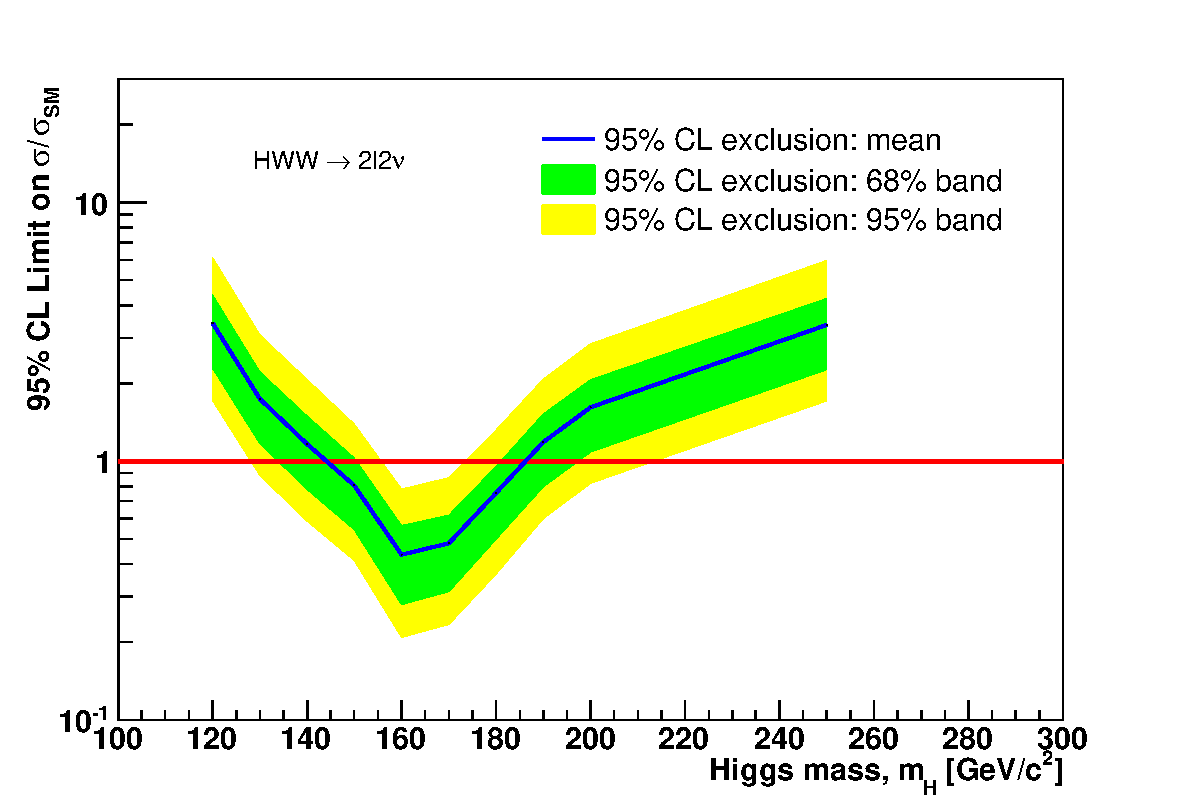
\includegraphics[width=0.9\textwidth]{figures/cut_based_limits.pdf}
   \caption{Cut based analysis expected upper limits at 95\%C.L. for 1\ifb\ of data.}
   \label{fig:cutbase_uls}
\end{center}
\end{figure}


\section{Summary}
    \label{sec:summary}
%    In summary, we described an analysis to study the spin of a single narrow 
resonance at 125 GeV by the gluon fusion through the decays into $WW\to 2\ell2\nu$.  
The analysis is based on a two-dimensional templates $m_T-m_{\ell\ell}$. 
The expected sensitivity to distinguish between between SM Higgs hypothesis and 
spin 2 Graviton like resonance with minimal coupling 
$2_\text{min}^+$ is $1.7\sigma$ for \intlumiEightTeV. 
Scaling by luminosity the projected separation is about $2.0\sigma$ for 25~$\ifb$. 


\clearpage



\appendix
\appendixpage
%%   \section{Anomalous triple gauge couplings}
%%     \label{app:atgc}
%%     \input{atgc}
%%   \section{Electron selection details}\label{sec:eledetail}
%%     \input{electron_detail}
%%   \section{Using the transverse mass of the $W$ for
%%     \dytt\ suppression}\label{sec:mt} 
%%     \input{mt}
%%   \section{Jet Veto at high $\eta$}
%%     \input{higheta}
%%   \section{Jet Veto using $b$ tagging}
%%     \input{btagging}
%%   \section{Application of the Drell-Yan estimate method}
%%     \label{app:dy22X}
%%     \input{drell_yan_appendix}
%%   \section{Event yields in other samples}
%%     \label{app:othersamples}
%%     \input{alt_samples}
%%   \section{Estimating the sensitivity to observe \ww\ in 100/pb}
%%     \label{app:significance}
%%     \input{significance}
%%   \section{QCD multi jet background estimation}
%%     \label{app:qcd}
%%     \input{qcd}
%% \clearpage

\vspace*{-0.2cm}
\thebibliography{12}

\bibitem{pdg}
 K. Nakamura et al. (Particle Data Group), "Review of particle physics", J. Phys.G37 , 2010.

\bibitem{Higgs1}
F. Englert and R. Brout, "Broken symmetries and the masses of gauge bosons", Phys. Rev. Lett. 13,  1964.

\bibitem{Higgs2}
P. W. Higgs, "Broken symmetry and the mass of gauge vector mesons", Phys. Rev. Lett. 13, 1964.

\bibitem{Higgs3}
Guralnik, G.S. and Hagen, C.R. and Kibble, T.W.B., "Global Conservation Laws and Massless Particles", 
Phys.Rev.Lett. 13, 1964.

\bibitem{HWW2010}
CMS Collaboration, "Title: Measurement of WW Production and Search for the Higgs Boson in 
pp Collisions at $\sqrt{s}$ = 7 TeV", arXiv:1102.5429

\bibitem{VBTFCrossSectionNote}
J. Alcaraz Maestre, \textit{et al.}, "Updated Measurements of Inclusive W and Z Cross Sections 
at $\sqrt{s}=7$ TeV", CMS AN-2010/264.

\bibitem{ggWWError}
F.~ Stoeckli, "http://indico.cern.ch/getFile.py/access?contribId=0\&resId=1\&materialId=slides\&confId=49009", 
EWK Diboson meeting of March 12 2009.

\bibitem{json}
{\small
/afs/cern.ch/cms/CAF/CMSCOMM/COMM\_DQM/certification/Collisions11/7TeV/Prompt/Cert\_160404-163869\_7TeV\_PromptReco\_Collisions11\_JSON.txt
}

\bibitem{ElIso}
A. Vartak, M. LeBourgeois, V. Sharma, "Lepton Isolation in the CMS Tracker, ECAL and HCAL", CMS AN-2010/106.

\bibitem{PVDA}
W. Erdmann, M. LeBourgeois, B. Mangano, 
https://indico.cern.ch/getFile.py/access?contribId=5\&sessionId=3\&resId=1\&materialId=slides\&confId=127127, 
note in preparation.

\bibitem{NExpHits}
B. Mangano \textit{et al.}, "Improvement in Photon Conversion Rejection Performance Using 
Advanced Tracking Tools", AN-10-283.

\bibitem{fakeLeptonNote1}
S.~Xie, \textit{et al.}", "Study of Data-Driven Methods for Estimation of Fake Lepton Backgrounds", 
CMS AN-2009/120.

\bibitem{fakeLeptonNote2}
W.~Andrews, \textit{et al.}, "Fake Rates for dilepton Analyses", CMS AN-2010/257.

\bibitem{fakeLeptonBkgSpillage1}
 F. Golf, D. Evans, J. Mulmenstadt  \textit{et al.}, ``Expectations for observation of top quark pair production in the dilepton final state with the early CMS data'', CMS AN-2009/050.

\bibitem{dyestnote}
W. Andrews, et al., “A Method to Measure the Contribution of $\dyll$ to a di-lepton+ MET Selection”, CMS AN-2009/023 (2009).

\bibitem{jes}
CMS Collaboration, "Jet Energy Calibration with Photon+Jet Events", PAS JME-09-004.

\bibitem{jetpas}
CMS Collaboration, "Jet Performance in pp Collisions at $\sqrt{s}=7 \rm\ TeV$", PAS JME-10-003.

\bibitem{btag}
CMS collaboration, "Commissioning of b-jet identification with pp collisions at $\sqrt{s}=7~\TeV$, BTV-10-001.

\bibitem{antikt}
Cacciari, Matteo and Salam, Gavin P. and Soyez, Gregory, "The anti-$k_t$ jet clustering 
algorithm", JHEP 04,  2008.

\bibitem{ConversionNote}
W.~Andrews, \textit{et al.}, "Study of photon conversion rejection at CMS", CMS AN-2009/159.

\bibitem{tmva}
A. Hoecker, \textit{et al.}, "TMVA - Toolkit for Multivariate Data Analysis", arXiv:physics/0703039, 2007.

\bibitem{XS}
CMS Generator group, Standard Model Cross Sections for CMS at 7 TeV, 2010.

\bibitem{PDF4LHC}
PDF4LHC Working Group, 
{\tt http://www.hep.ucl.ac.uk/pdf4lhc/PDF4LHCrecom.pdf}

\bibitem{Nadolsky:2008zw}
Nadolsky, Pavel M. and others, "Implications of CTEQ global analysis for 
collider observables", Phys. Rev. D78 2008.

\bibitem{Martin:2009iq}
Martin, A. D. and Stirling, W. J. and Thorne, R. S. and Watt, G., "Parton 
distributions for the LHC, Eur. Phys. J. C63 2009.

\bibitem{Ball:2010de}
Ball, Richard D. and others, "A first unbiased global NLO determination 
of parton distributions and their uncertainties", arXiv 1002.4407.

\bibitem{bayesian}
A. O'Hagan and J.J. Forster, "Bayesian Inference", Kendall's Advanced Theory of Statistics, 
Arnold, London, 2B, 2004.

\bibitem{ref:tagprobe_mit_w}
G. Bauer {\it et. al.}, "Lepton ef?iencies for the inclusive W cross section measurement with 36.1pb$^{-1}$", AN2011/097

\bibitem{ref:tagprobe_snt_top}
W. Andrews {\it et. al.}, "Uncertainties on the Lepton Selection Efficiency for t$t\bar{t}$ Cross Section Analysis", AN2010/274

\bibitem{LHCHiggsCrossSectionWorkingGroup:2011ti}
LHC Higgs Cross Section Working Group, "Handbook of LHC Higgs Cross Sections: 
Inclusive Observables", CERN-2011-002, 2011.

\bibitem{PFMET} 
CMS Collaboration, ``CMS MET Performance in Events Containing Electroweak Bosons from pp Collisions at $\sqrt{s}=7$ TeV'', CMS PAS JME-2010-005 (2010)


\bibitem{trkMET} 
Marco Zanetti, ``MET with PU in $\hww\to2\ell$'', https://indico.cern.ch/conferenceDisplay.py?confId=131580
Benjamin Hooberman, ``MET with PU in MC and First 2011 Data'', https://indico.cern.ch/contributionDisplay.py?contribId=5\&confId=132579. 


\bibitem{lands}
Mingshui Chen and Andrey Korytov, https://mschen.web.cern.ch/mschen/lands/

\bibitem{MCFMHiggsProduction}
J. Campbell, R.K. Ellis, G. Zanderighi, ``Next-to-Leading order Higgs + 2 jet production via gluon fusion.'', JHEP 0610:028 (2006), hep-ph/0608194

\end{document}
